\documentclass[
    % draft,
]{sotsu}

\usepackage{ifdraft}

\usepackage{sotsu}
\usepackage{sotsu-symb}
\usepackage{sotsu-thm}

\crefname{equation}{式}{式}

\usepackage{tcolorbox}
\tcbuselibrary{skins}
\NewTColorBox[auto counter]{qmaxiom}{O{}}{
    enhanced jigsaw,
    fonttitle={\bfseries\gtfamily\sffamily},
    title={公理~\thetcbcounter.},
    opacityback=0, % standard jigsaw
    attach boxed title to top left={yshift=-2mm},
}

\usepackage[
    style=sotsu,
    maxnames=99,
    minnames=99,
    ]{biblatex}
\addbibresource{sotsu.bib}


\ModifyHeading{subsubsection}{
    label_format={\thesubsubsection},
    lines=2,
    font={\large\sffamily\gtfamily\bfseries},
    format={%
        \jlreqHeadingLabel{{\rmfamily\mcfamily\bfseries \thesubsubsection} \quad}%
        #2%
    },
}


% 仮コマンド
\newcommand{\bpsi}{\symbf{\psi}}
\newcommand{\bphi}{\symbf{\varphi}}
\newcommand{\bxi}{\symbf{\xi}}


\definecolor{fire}{RGB}{255, 90, 0}
\definecolor{water}{RGB}{0, 120, 255}

\newcommand{\fire}[1]{\textcolor{fire}{#1}}
\newcommand{\water}[1]{\textcolor{water}{#1}}


\title{量子力学的なにか}
\date{\today}


\ExplSyntaxOn
\makeatletter
\renewcommand{\maketitle}{
    \begin{titlepage}
        \null\vfil
        \centering
        {\LARGE \@title}
        \par
        {\large \@date}
        \vfil\null
        \par
        \ifdraft{}{
        \begin{minipage}{0.7\linewidth}
            \begin{minipage}{0.2\linewidth}
                \centering
                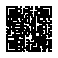
\includegraphics[width=2cm]{misc/github_url.pdf}
            \end{minipage}
            \hfil
            \begin{minipage}{0.7\linewidth}
                PDFファイルと\LaTeX ソースは,
                \url{https://github.com/scasc1939/nusotsu}で配布しています.
            \end{minipage}
            \vskip 1cm
            \begin{minipage}{0.2\linewidth}
                \centering
                
\includegraphics[width=2cm]{misc/cc-by-sa.pdf}
            \end{minipage}
            \hfil
            \begin{minipage}{0.7\linewidth}
                This~work~is~licensed~under~CC~BY-SA~4.0.
                \\
                \url{https://creativecommons.org/licenses/by-sa/4.0/}
            \end{minipage}
        \end{minipage}
        }
    \end{titlepage}
}
\makeatother
\ExplSyntaxOff


\begin{document}

\maketitle

\tableofcontents

\clearpage



\section{イントロダクション}

17世紀から18世紀にかけての物理学者,ニュートンが大成した古典力学(ニュートン力学)によって,
物体の運動は完全に記述できるようになった.
この世界は原子という物体によって構成されているのだから\footnote{
    実は,原子の存在が証明されたのは1905年.
    アインシュタインによるブラウン運動の解明による.
},
現時点での宇宙の全原子の座標と運動量(および相互作用)を完全に決定できる存在,
いわゆる\emph{ラプラスの悪魔}は,
この世界の過去も未来もすべて知ることができる.
のちに形成された解析力学のことばを使えば,
各原子のハミルトニアンと初期状態が,その原子の時間発展を決定する%
%(また正準方程式は時間反転に対して対称である),
といえる.

もちろん実際には,
宇宙の全原子はおろか,
小さな箱に閉じ込められた気体を構成する全原子の座標と運動量を特定することすら,
人間には不可能である.
このような多数------おおよそ$10^{23}$個のオーダー-----の原子がつくる\emph{多体系}は,
各粒子を支配しているはずのニュートン力学からは想像もつかないようなふるまいを示す.
ニュートン方程式は可逆であるにもかかわらず,
多体系は本質的に不可逆的である.
実際,熱湯と水を混ぜればぬるま湯になるが,
逆にぬるま湯が熱湯と水に分離されるところを見た人はいないだろう.
このような「\emph{マクロ}な世界」を扱うのが\emph{統計力学}である.
ニュートン力学には存在しない「温度」や「エントロピー」といった概念が,
統計力学において定義されることは,
よく知られている.

マクロな理論である統計力学の形成から少し遅れた20世紀初頭,
\emph{ミクロ}な世界の理論である\emph{量子力学}が形成された.
量子力学によればエネルギーは離散的な値しかとることができないし,
物理量は確率的にしか予言できず,
さらには状態を重ね合わせることができる.
また,そこで扱われる量子力学的粒子も,
古典粒子に存在しない「スピン」や「位相」といった値を持つ.
このような点で,量子力学は古典力学と根本的に異なる理論体系である.
しかしながら,面白いことに,視野を広げる(ミクロな世界から遠ざかる)ことで,
量子力学は古典力学に漸近するのである.
水素原子のスペクトル問題は,
量子力学によって見事に解き明かされた.


1905年にはアインシュタインが特殊相対論を提唱し,
絶対時間の存在を暗黙裡に仮定していたニュートン力学はここに崩壊した.
量子力学を相対論的に書き直す試みがなされるまで,
それほど時間はかからなかった.
1928年,ディラックは,量子力学に相対論的効果を導入したディラック方程式を提唱した.
この方程式からは,
すべての粒子に対して,
質量が同じで,電荷の符号が逆である粒子(\emph{反粒子})が存在することが示唆される.
反粒子が実在することは,
1932年のアンダーソンによる陽電子の発見によって裏付けられた.


量子力学を使って統計力学を捉えなおすこともなされた.
すなわち,多体系を構成する粒子が量子力学的であるとするのである.
一切の相互作用なくしておこる相転移,
ボース・アインシュタイン凝縮はまさに量子統計力学の醍醐味である.


1911年,カメルリング・オネス\footnote{
    Kamerlingh Onnesのカタカナ表記は,
    状態密度$D$・$N$問題,
    ボーズ・ボース問題,
    Liouvilleの読み方問題と並ぶ統計力学の難問である.
}は極低温に冷やした水銀の電気抵抗がゼロになることを発見した.
のちに超伝導と呼ばれるこの現象の理論的解明は,
1957年にバーディーン,クーパー,シュリーファーによってなされた.
3人の頭文字をとってBCS理論と呼ばれるこの理論は,
量子力学を多体系に適用したものである.


このように,量子力学を応用することによって多くの新奇的な物理現象が明らかになったわけであるが,
しかしその中で量子力学の数学的位置づけは等閑視されてきた.
これを読んでいる人でヒルベルト空間を知らない人はいないだろうが,
ではヒルベルト空間の定義を述べよ,といわれると動揺する人が多いのではないだろうか.
むろん基礎から量子力学を理解するよりも,
実際に量子力学を使って物理現象を理解することが重要であるという考え方も大いにあり得よう.
量子力学の厳密な数学的定式化はフォン・ノイマン(1932年)によってなされた.







\section{ヒルベルト空間の定義}

量子状態はヒルベルト空間の元であるベクトルによって記述される.
そこで,この節ではまず,一般のヒルベルト空間について定義する.
スピン系のような有限次元のヒルベルト空間のベクトルとは,
単なる数ベクトルであることを示す.


\subsection{ベクトル空間}

量子力学は線形代数である,
量子力学的状態はベクトルであるというのはよく言われることである.
このことを理解するために,
まずはベクトルとは何かをきちんと定義することにしよう.


\subsubsection{ベクトル空間の定義}
\label{sec:definition-of-vector-space}

まずは\emph{ベクトル空間}を定義する.
$\symbb{C}$を複素数全体の集合とする.
集合$V$があって,
$V$の\ltjruby{元}{げん}に対して\emph{和}$\vecplus \colon V \times V \to V$,
\emph{スカラー倍}$\scaprod \colon \symbb{C} \times V \to V$が定義されているとする.
$V$の元を$\bpsi, \bphi, \bxi$,
複素数$a, b$としたとき,
以下の8条件
\begin{enumerate}
    \item \label{vector:sum-associative}
        \bluehead{和は結合的である}------すなわち,
        \fire{任意の$\bpsi, \bphi, \bxi \in V$}に対し,
        $(\bpsi \vecplus \bphi) \vecplus \bxi = \bpsi \vecplus (\bphi \vecplus \bxi)$.
    \item \label{vector:sum-commutative}
        \bluehead{和は交換する}------すなわち,
        \fire{任意の$\bpsi, \bphi, \bxi \in V$}に対し,
        $\bpsi \vecplus \bphi = \bphi \vecplus \bpsi$.
    \item \label{vector:sum-zero}
        \bluehead{和に対する零元の存在}------すなわち,
        \water{ある$\symbf{0} \in V$}が存在して,
        \fire{任意の$\bpsi \in V$}に対し,$\bpsi \vecplus \symbf{0} = \bpsi$.
    \item \label{vector:sum-opposite}
        \bluehead{和に対する逆元の存在}------すなわち,
        \fire{任意の$\bpsi \in V$}に対し,
        \water{ある$\bphi \in V$}が存在して,
        $\bpsi \vecplus \bphi = \symbf{0}$.
    \item \label{vector:scalar-sum}
        \bluehead{スカラー倍は複素数の和に対して分配的である}------すなわち,
        \fire{任意の$\bpsi \in V$}と\fire{任意の複素数$a, b$}に対し,
        $(a + b) \scaprod \bpsi = (a \scaprod \bpsi) + (b \scaprod \bpsi)$.
    \item \label{vector:scalar-distributive}
        \bluehead{スカラー倍は$V$上の和に対して分配的である}------すなわち,
        \fire{任意の$\bpsi, \bphi \in V$}と\fire{任意の複素数$a$}に対し,
        $a \scaprod (\bpsi \vecplus \bphi) = (a \scaprod \bpsi) \vecplus (a \scaprod \bphi)$.
    \item \label{vector:scalar-prod}
        \bluehead{複素数の積とスカラー倍の結合}------すなわち,
        \fire{任意の$\bpsi \in V$}と\fire{任意の複素数$a, b$}に対し,
        $(ab) \scaprod \bpsi = a \scaprod (b \scaprod \bpsi)$.
    \item \label{vector:scalar-identity}
        \bluehead{$1$はスカラー倍の単位元}------すなわち,
        複素数$1$について,\fire{任意の$\bpsi \in V$}に対し,
        $1 \scaprod \bpsi = \bpsi$.
\end{enumerate}
を満たすのならば,
$V$を\ltword{ベクトル空間}(vector space)と呼び,
$V$の元(上で挙げた$\bpsi, \bphi, \bxi, \dotsc$)を\ltword{ベクトル}という.

ここで,上の条件に出てくる「\fire{任意の}---」と「\water{ある}---」の順序は重要である.
\labelcref*{vector:sum-zero}では$\symbf{0}$はただひとつであり,
その$\symbf{0}$について$\bpsi \vecplus \symbf{0} = \bpsi$が満たされ,
さらに$\bphi \vecplus \symbf{0} = \bphi$が成り立たねばならない.
その一方で,\labelcref*{vector:sum-opposite}における$\bphi$は,
$\bpsi$のとりかたによって変わりうる.
あるベクトル$\bpsi$に対して$\bpsi \vecplus \bphi = \symbf{0}$が満たされても,
別のベクトル$\bxi$に対して$\bxi \vecplus \bphi = \symbf{0}$が成り立つとは限らない.



\subsubsection{ベクトル空間の例}
\label{sec:example-of-vector-space}

\bluehead{ユークリッド空間}\quad
ベクトル空間の典型例は\word{ユークリッド空間}(Euclidean space)である.
ある自然数$N$($\geq 1$)に対し,
集合$\symbb{C}^N$を
\begin{equation*}
    \symbb{C}^N 
    \coloneq
    \Set*{
    \symbf{x} = 
    \begin{pmatrix}
        x_1  \\  \vdots  \\  x_N
    \end{pmatrix}
    \given 
    \text{$x_1, \dots, x_N$は複素数}
    }
\end{equation*}
で定める.
和$\vecplus$とスカラー倍$\scaprod$は,
各成分の和と積,つまり
\begin{align*}
    \symbf{x} \vecplus \symbf{y}
        &\coloneq 
        \begin{pmatrix}
            x_1 + y_1  \\
            \vdots     \\
            x_N + y_N
        \end{pmatrix},
    \quad
    c \scaprod \symbf{x}
        \coloneq 
        \begin{pmatrix}
            c x_1  \\
            \vdots \\
            c x_N
        \end{pmatrix}
\end{align*}
で定める.
このとき,$\symbb{C}^N$がベクトル空間の定義を満たすことを確認するのは容易である.
まず,
\cref{vector:sum-associative,vector:sum-commutative}は,
複素数の性質から明らかである.
\cref{vector:sum-zero}における$\symbf{0}$は,
\begin{equation*}
    \symbf{0} \coloneq 
    \begin{pmatrix}
        0  \\  \vdots  \\  0
    \end{pmatrix}
\end{equation*}
で与えられる.
また,\cref{vector:sum-opposite}でいう,$\symbf{x}$に対して$\symbf{x} \vecplus \symbf{y} = \symbf{0}$を満たすベクトル
$\symbf{y}$は,
\begin{equation*}
    \symbf{y} \coloneq 
    -\symbf{x} =
    \begin{pmatrix}
        -x_1  \\  \vdots  \\  -x_N
    \end{pmatrix}
\end{equation*}
である.
\cref{vector:scalar-sum,vector:scalar-distributive}は複素数の分配法則に帰着されるし,
\cref{vector:scalar-prod}は複素数の結合法則そのものである.
\cref{vector:scalar-identity}は複素数$1$が乗法の単位元であることから直ちに従う.

以上のことから$\symbb{C}^N$がベクトル空間であることが示されたが,
実は\cref{sec:definition-of-vector-space}で与えたベクトル空間の定義は,
この$\symbb{C}^N$が満たす性質を抽出して羅列したものである.
物理学の教科書で「具体例から基本法則を導く」ことが多いのとは対照的に,
数学ではこのような「一般から具体」という論理展開が好まれる\footnote{
    上のように,具体例を与えずに初めに定義を書くことは,
    物理では「\ltjruby{天|下}{あま|くだ}り的」とされて忌避される傾向にある.
}.
しかし,論理の形式としては一般から具体であっても,
たいていは抽象的な定義のもととなった典型例が存在する.
今回の場合,抽象的に定義された「ベクトル空間」の典型例がユークリッド空間である.


\bluehead{$N$階斉次線形常微分方程式の解空間}\quad
$N$階\footnote{
    \ltjruby{$N$|階}{|かい}とは,
    方程式に含まれる未知関数$y(x)$の導関数$y^{(n)}$のうち,
    もっとも高い階数が$N$であることをいう.
}の斉次\footnote{
    \ltjruby{斉|次}{せい|じ}とは,未知関数$y(x)$とその導関数$y^{(n)} (x)$を含まない項$f(x)$が存在しないことをいう.
}線形\footnote{
    微分方程式における\ltjruby{線|形}{せん|けい}とは,
    未知関数$y(x)$とその導関数$y^{(n)} (x)$について,
    2次以上の項($2 (y')^2$のような)が存在しないことをいう.
}方程式
\begin{equation}
    \label{eq:N-differential-equation}
    a_N (x) \dv[N]{y}{x} + a_{N-1} (x) \dv[N-1]{y}{x}
        + \dots + a_2 (x) y'' + a_1 (x) y' + a_0 (x) y = 0
    \quad (a_N \neq 0)
\end{equation}
には,
互いに独立である解が$N$個存在することが知られている.
そこで,それらを$\varphi_1 (x), \dots, \varphi_N (x)$とおくと,
任意の複素数$c_1, \dots, c_N$に対して$y(x) = c_1 \varphi_1 (x) + \dots + c_N \varphi_N (x)$はこの微分方程式の解になっている.
関数の和$y_1 (x) + y_2 (x)$とスカラー倍$c y(x)$がベクトル空間の条件を満たすことは,
\cref{vector:sum-zero}における$\symbf{0}$が関数としてのゼロ$y(x) \equiv 0$であることに注意すれば,
ほとんど自明である.

1次元の時間に依存しないシュレーディンガー方程式
\begin{equation}
    \label{eq:Schroedinger}
    -\frac{\hbar^2}{2m} \dv[2]{\psi(x)}{x} + V(x) \psi(x) = E \psi(x)
\end{equation}
は2階の斉次線形常微分方程式である.
無限に深い井戸型ポテンシャル
\begin{equation*}
    V(x) = 
    \begin{cases}
        0      &  0 \leq x \leq L  \\
        \infty &  \text{others}
    \end{cases}
\end{equation*}
の場合の2つの独立な解が
\begin{equation*}
    \varphi_{\pm} (x) = 
    \begin{cases}
        \exp \ab(\pm \frac{\sqrt{2 m E}}{\hbar})  &  0 \leq x \leq L  \\
        0  &  \text{others}
    \end{cases}
\end{equation*}
であることはよく知られている.
任意の複素数$c_1, c_2$に対して$\psi(x) = c_1 \varphi_{+} (x) + c_2 \varphi_{-} (x)$もまた\cref{eq:Schroedinger}の解になっていることも明らかであろう.



\bluehead{関数空間}\quad
もう少し特殊なベクトル空間として,
関数のなす空間を考えよう.
実数係数の\ltword{多項式空間}$\symbb{R}[x]$を
\begin{equation*}
    \symbb{R}[x] \coloneq 
    \Set*{ \sum_{i=1}^{n} c_i x^i
        \given
        \begin{array}{c}
            \text{$c_1, \dots, c_n$は実数}  \\
            \text{$n = 0, 1, 2, \dots$}
        \end{array}
        }
\end{equation*}
で定義する.
$\symbb{R}[x]$がベクトル空間になっていることもすぐにわかる.
例えば多項式の和はまた多項式であるし,
多項式のスカラー倍(つまり,全体に数$c$をかけたもの)も多項式である\footnote{
    本来は「多項式の和$\vecplus$とスカラー倍$\scaprod$を定義しないといけないが,
    煩雑さを避けるため割愛する.
}.
\cref{sec:definition-of-vector-space}の8条件を満たすことは,
これらの演算が\cref{vector:sum-zero}の$\symbf{0}$が多項式としての$0$であることに注意すれば,
ほとんど自明である.
$\symbb{R}[x]$に属するベクトルの例は,
$2x$, $3x^3 - \sqrt{2} x + 1$などである.

同様にして,連続関数全体$C^0$や,
$n$回微分可能な関数全体$C^n$もベクトル空間であることが示される.
このような事実を踏まえて,
量子力学的状態$\bpsi(x)$がベクトルであるといっているのである.



\subsection{基底と次元}

\subsubsection{有限個の基底}

ベクトル空間の和とスカラー倍について,
進んだ考察をしてみよう.

考えるベクトル空間を$V$とする.
ベクトル空間の公理(より正確には,和とスカラー倍の定義)から,
$V$のベクトル$\symbf{u}_1, \dots, \symbf{u}_n$と複素数$c_1, \dots, c_n$に対して,
\begin{equation}
    \label{eq:linear-combination}
    \symbf{v} \coloneq c_1 \symbf{u}_1 + \dots + c_n \symbf{u}_n
\end{equation}
で定義される$\symbf{v}$はまた$V$のベクトルになる.
そこで\cref{eq:linear-combination}のことを,
ベクトル$\symbf{u}_1, \dots, \symbf{u}_n$の\ltword{線形結合}(linear combination)という.
線形結合はベクトル空間論の基礎をなす重要概念であり,
ある意味ベクトルの本質ともいえる.
ベクトル空間における概念の多くが,
この線形結合を用いて定義される.
以下でその例を見てみよう.

ベクトルの組$\symbf{u}_1, \dots, \symbf{u}_n \in V$が,
複素数$c_1, \dots, c_n$に対して
\begin{equation}
    \label{eq:linearly-independent}
    \symbf{0} = c_1 \symbf{u}_1 + \dots + c_n \symbf{u}_n
\end{equation}
を満たすとする.
\cref{eq:linearly-independent}のことを$\symbf{u}_1, \dots, \symbf{u}_n$の\ltword{一次関係}(linear relation)という.
もし$c_1 = \dots = c_n = 0$ならば,
\cref{eq:linearly-independent}は当然成り立つ.
逆に,\cref{eq:linearly-independent}が成り立つのが$c_1 = \dots = c_n = 0$の場合に限るとき,
$\symbf{u}_1, \dots, \symbf{u}_n$は\ltword{一次独立}(linearly independent)であるという.

また,$V$のベクトル$\symbf{u}_1, \dots, \symbf{u}_n$の線形結合の全体が$V$に一致する,
つまり
\begin{equation*}
    V = \Set{
            c_1 \symbf{u}_1 + \dots + c_n \symbf{u}_n
            \given
            \text{$c_1, \dots, c_n$は複素数}
            }
\end{equation*}
であるとき,$\symbf{u}_1, \dots, \symbf{u}_n$は$V$を\ltword{生成する}という.
あるいは$V$のすべてのベクトルが\cref{eq:linear-combination}の形で書けるといってもよい.

ここまでの準備によって,
基底という概念を定義できる.
$\symbf{u}_1, \dots, \symbf{u}_n$を$V$のベクトルとする.
以下の2条件
\begin{enumerate}
    \item $\symbf{u}_1, \dots, \symbf{u}_n$は一次独立である.
    \item $\symbf{u}_1, \dots, \symbf{u}_n$は$V$を生成する.
\end{enumerate}
が満たされるとき,
$\symbf{u}_1, \dots, \symbf{u}_n$は$V$の\ltword{基|底}[き|てい](basis)であるという.

\bluehead{$\symbb{C}^N$の基底}\quad 
例えば,$V$をユークリッド空間$\symbb{C}^N$としよう.
$V$の基底は,例えば
\begin{equation}
    \label{eq:Euclidean-basis-1}
    \symbf{e}_1 \coloneq
    \begin{pmatrix}
        1  \\  0  \\  0  \\  \vdots  \\  0
    \end{pmatrix}
    , \quad
    \symbf{e}_2 \coloneq
    \begin{pmatrix}
        0  \\  1  \\  0  \\  \vdots  \\  0
    \end{pmatrix}
    , \quad \dotsc, \quad
    \symbf{e}_N \coloneq
    \begin{pmatrix}
        0  \\  0  \\  \vdots  \\  0  \\  1
    \end{pmatrix}
\end{equation}
が考えられる.
$\symbf{e}_1, \dots, \symbf{e}_N$が$V$を生成することは,
$\symbb{C}^N$の任意のベクトル$\symbf{x}$が
\begin{equation*}
    \symbf{x}
    \equiv
    \begin{pmatrix}
        c_1  \\  c_2  \\  \vdots  \\  c_N
    \end{pmatrix}
    =
    c_1 \symbf{e}_1 + c_2 \symbf{e}_2 + \dots + c_N \symbf{e}_N
\end{equation*}
(ただし$c_1, c_2, \dots, c_N$は任意の複素数)とあらわされることからわかる.
また,一次独立性は,
\begin{equation*}
    \symbf{0} 
        \equiv
        \begin{pmatrix}
            0  \\  0  \\  \vdots  \\  0
        \end{pmatrix}
        = c_1 \symbf{e}_1 + c_2 \symbf{e}_2 + \dots + c_N \symbf{e}_N
        \equiv
        \begin{pmatrix}
            c_1  \\  c_2  \\  \vdots  \\  c_N
        \end{pmatrix}
\end{equation*}
より$c_1 = c_2 = \dots = c_N = 0$と確認される.

ところで,
\cref{eq:Euclidean-basis-1}は$\symbb{C}^N$の\emph{唯一の}基底ではない.
実際,$\symbb{C}^N$には別の基底が存在して,
たとえば
\begin{equation}
    \tag{\ref*{eq:Euclidean-basis-1}$'$}
    \label{eq:Euclidean-basis-2}
    \symbf{e}'_1 \coloneq
    \begin{pmatrix}
        1  \\  -1  \\  0  \\  \vdots  \\  0  \\  0
    \end{pmatrix}
    , \quad
    \symbf{e}'_2 \coloneq
    \begin{pmatrix}
        0  \\  1  \\  -1  \\  0  \\  \vdots  \\  0
    \end{pmatrix}
    , \quad \dotsc, \quad
    \symbf{e}'_{N-1} \coloneq
    \begin{pmatrix}
        0  \\  0  \\  \vdots  \\  0  \\  1  \\  -1
    \end{pmatrix}
    , \quad
    \symbf{e}'_N \coloneq
    \begin{pmatrix}
        0  \\  0  \\  \vdots  \\  0  \\  0  \\  1
    \end{pmatrix}
\end{equation}
は基底になっている.
これらが一次独立であることは,
$c_1 \symbf{e}'_1 + \dots + c_N \symbf{e}'_N = \symbf{0}$とおくことで,
\begin{equation*}
    c_1 = 0, 
    \quad 
    c_2 - c_1 = 0, 
    \quad
    \dotsb,
    \quad 
    c_{N-1} - c_N = 0,
    \quad
    c_N = 0
\end{equation*}
という連立不等式が得られ,
ここから$c_1 = c_2 = \dots = c_N = 0$が従うことよりわかる.
また$V$を生成することは,
任意のベクトル$\symbf{x} = \cvector{x_1 ; x_2 ; \cdots ; x_N} \in V$が
\begin{equation*}
    \symbf{x} \equiv 
    \begin{pmatrix}
        x_1  \\  x_2  \\  \vdots  \\  x_N
    \end{pmatrix}
    =
      x_1 \symbf{e}'_1
    + (x_2 + x_1) \symbf{e}'_2
    + \dotsb 
    + (x_{N-1} + x_{N-2}) \symbf{e}'_{N-1}
    + (x_{N-1} + x_N) \symbf{e}'_{N-1}
\end{equation*}
と表せることから従う.


\subsubsection{無限個の基底}
\label{sec:infinite-basis}

今までの議論では,
基底が有限個の場合についてのみ考えていた.
ここでは基底が無限個ある場合を考える.
そのためには,
線形結合の定義を拡張する必要がある.

以降,表記を簡単にするために,
可算無限(自然数$\symbb{N}$と同じくらいの数)の場合についてだけ考える.
物理学で扱うヒルベルト空間は,
無限次元であっても可分である(\ltjruby{稠|密}{ちゅう|みつ}な高々可算集合をもつ)ので,
この仮定を行っても特に支障はない.

考えるベクトル空間を$V$とする.
$V$のベクトル$\symbf{u}_1, \symbf{u}_2, \dots$に対して,
\begin{equation}
    \label{eq:infinite-linear-combination}
    \symbf{v} \coloneq
    \sum_{i = 1}^{\infty} c_i \symbf{u}_i,
    \quad
    \text{ただし$c_1, c_2, \dots$は有限個を除きゼロである複素数}
\end{equation}
で定義される$V$のベクトル$\symbf{v}$を,
$\symbf{u}_1, \symbf{u}_2, \dots$の\ltword{線形結合}という.

ここで,無限個の複素数$c_1, c_2, \dots$が有限個を除きゼロである,つまり\cref{infinite-linear-combination}が実は
\begin{equation*}
    \symbf{v} = c_{i_1} \symbf{u}_{i_1} + \dots + c_{i_n} \symbf{u}_{i_n}
\end{equation*}
という有限の和でかけるという条件は必要不可欠である.
実際,和が有限でない場合,
すべての$i$に対して$\symbf{u}_i \in V$でも,
$\sum_{i=1}^{\infty} c_i \symbf{u}_i \notin V$となることがあり得る.
例えば関数$1, x, x^2, \dots, x^n, \dots$はすべて多項式関数であるが,
それらの``線形結合''
\begin{equation}
    \label{eq:exponential-expansion}
    1 + x + \frac{1}{2!} x^2 + \dots + \frac{1}{n!} x^n + \dotsb = e^x
\end{equation}
は多項式関数でない.

ベクトル空間$V$に属するベクトル$\symbf{u}_1, \symbf{u}_2, \dots$が\ltword{一次独立}であるとは,
\fire{有限個を除きゼロである}複素数の組$c_1, c_2, \dots$を用いて
\begin{equation*}
    \symbf{0} = \sum_{i = 1}^{\infty} c_i \symbf{u}_i
\end{equation*}
と書けたなら,$c_1 = c_2 = \dots = 0$が成り立つことをいう.
また,
$\symbf{u}_1, \symbf{u}_2, \dots$が$V$を\ltword{生成する}とは,
すべての$V$のベクトル$\symbf{v}$がそれらの線形結合で書ける,
つまり\fire{有限個を除きゼロである}複素数の組$c_1, c_2, \dots$を用いて
\begin{equation*}
    \symbf{v} = \sum_{i = 1}^{\infty} c_i \symbf{u}_i
\end{equation*}
が成り立つことをいう.
$\symbf{u}_1, \symbf{u}_2, \dots$が$V$の\ltword{基底}であるとは,
これらが一次独立であり,
かつ$V$を生成することをいう.





\subsubsection{ベクトル空間の基底と次元}

ベクトル空間が与えられても,
その基底の取り方には任意性がある.
たとえば\cref{eq:Euclidean-basis-1}と\cref{eq:Euclidean-basis-2}は,
ともにユークリッド空間$\symbb{C}^N$の基底をなす.
しかし,基底を構成するベクトルの数は,
どのような基底をとっても常に一定である.
実際,\cref{eq:Euclidean-basis-1},\cref{eq:Euclidean-basis-2}は,
ともに$N$個のベクトルからなる.
これを証明しよう.

あるベクトル空間$V$に対して,
基底$\sequ{\symbf{u}_i} \coloneq \symbf{u}_1, \dots, \symbf{u}_M$と,
基底$\sequ{\symbf{u}'_j} \coloneq \symbf{u}'_1, \dots, \symbf{u}'_N$がとれたとする.
まず$\sequ{\symbf{u}_i}$は$V$の基底であるから,
任意の$\symbf{u}'_j$は$\sequ{\symbf{u}_i}$の線形結合で書ける:
\begin{equation*}
    \symbf{u}'_j = \sum_{j = 1}^{M} c_{ij} \symbf{u}_i
    \quad ( 1 \leq i \leq N )
\end{equation*}
ここでもし$M < N$なら,
$\sequ{\symbf{u}'_j}$は一次従属になる.
なぜなら,複素数$a_1, \dots, a_N$を用いた$\sequ{\symbf{u}'_j}$の一次関係は
\begin{equation*}
    \begin{split}
        \symbf{0} &= \sum_{j = 1}^{N} a_j \symbf{u}'_j
            = \sum_{i = 1}^{M} \sum_{j = 1}^{N} a_j c_{ij} \symbf{u}_i
            \\
            &= 
            \begin{pmatrix}
                \symbf{u}_1  &  \cdots  &  \symbf{u}_M
            \end{pmatrix}
            \begin{pmatrix}
                c_{11}  &  \cdots  &  c_{1N}  \\
                \vdots  &  \ddots  &  \vdots  \\
                c_{M1}  &  \cdots  &  c_{MN}
            \end{pmatrix}
            \begin{pmatrix}
                a_1  \\  \vdots  \\  a_N
            \end{pmatrix}
    \end{split}
\end{equation*}
と書けるが,
行列の方程式
\begin{equation*}
    \begin{pmatrix}
        c_{11}  &  \cdots  &  c_{1N}  \\
        \vdots  &  \ddots  &  \vdots  \\
        c_{M1}  &  \cdots  &  c_{MN}
    \end{pmatrix}
    \symbf{a}
    =
    \symbf{0}
\end{equation*}
は$M < N$($\text{行数} < \text{列数}$)のとき必ず非自明な解$\symbf{a} \neq \symbf{0}$を持つからである.
仮定より$\sequ{\symbf{u}'_j}$は一次独立であるから,
$M \geq N$である.
同様の議論は$\sequ{\symbf{u}_i}$と$\sequ{\symbf{u}'_j}$を入れ替えても成立するので,
$N \geq M$である.
よって$M = N$であるといえる.

ベクトル空間$V$について,
その基底を構成するベクトルの数を,
$V$の\ltword{次|元}[じ|げん](dimension)という.
たとえば\cref{eq:Euclidean-basis-1}よりユークリッド空間$\symbb{C}^N$の次元は$N$である.
このような基底を構成するベクトルが有限個である空間は\ltword{有限次元}であるという.
そうでない空間は\ltword{無限次元}と呼ばれる.

\cref{sec:isomorphic}で議論するとおり,
有限次元のベクトル空間は実質的には$\symbb{C}^N$と同じものであり,
そこでの議論は行列と数ベクトルを用いた議論に置き換えることができる.
一方で無限次元のベクトル空間では,
行列を使った線形代数の議論は破綻する.
このような無限次元の線形代数を議論するのが\emph{関数解析学}とよばれる分野であるが,
これを学ぶには多くの前提知識が必要である.
量子力学の難しさには物理的な面と技術的な面とがあるが,
そのうちの後者にあたるのが,無限次元の議論である.

なお,古典的な状態(座標や運動量など)の張る空間は無限次元であるが,
純粋な量子力学的状態(スピンなど)では有限次元になる.
そこで,本稿では考える系をスピン系に限ることで,
無限次元の空間における面倒な問題を避け,
単純な行列計算を用いた議論を行うことにする.



\subsubsection{ベクトルの基底による分解}
\label{sec:expansion-of-basis}

$V$を有限次元のベクトル空間とし,
その基底として$\symbf{u}_1, \dots, \symbf{u}_N$をとる.
基底は$V$を生成するので,
$V$の任意のベクトル$\symbf{v}$は,
複素数の組$c_1, \dots, c_N$を用いて
\begin{equation*}
    \symbf{v} = c_1 \symbf{u}_1 + \dots + c_N \symbf{u}_N
\end{equation*}
とかける.
このとき,
基底$\symbf{u}_1, \dots, \symbf{u}_N$に対して,
係数$c_1, \dots, c_N$は一意に決まる.
それを確かめるために,
$\symbf{v}$が
\begin{equation*}
    \symbf{v} = c_1  \symbf{u}_1 + \dots + c_N  \symbf{u}_N
              = c'_1 \symbf{u}_1 + \dots + c'_N \symbf{u}_N
\end{equation*}
と2とおりに分解できたとしよう.
このとき,
ふたつめの等号およびベクトル空間の公理\cref{vector:scalar-sum}より
\begin{equation*}
    \symbf{0} = (c_1 - c'_1) \symbf{u}_1 + \dots + (c_N - c'_N) \symbf{u}_N
\end{equation*}
が成立する.
ここで基底は一次独立(\cref{eq:linearly-independent}を参照)であるので,
$c_1 - c'_1 = \dots = c_N - c'_N$が従う.
よって$c_1 = c'_1, \  \dots, \  c_N = c'_N$であるから,
結局$c_1, \dots, c_N$は1とおりに定まる.

無限次元空間のベクトルに対しても,
やはり基底を固定した時の展開係数は一意に定まる.
これを証明するのは難しくないが,
技術的に面倒であるのでここでは省略する.
なお,無限次元の量子力学でベクトルを展開するときには,
ふつうは基底ではなく\emph{完全正規直交系}を用いる.
完全正規直交系とよく似た概念に,
\cref{sec:ONB}で取り上げる\emph{正規直交基底}があるが,
前者は\cref{eq:linear-combination}での無限和を容認し,
後者は容認しない点で違いがある.



\subsubsection{基底の存在定理}

さて,ここまでベクトル空間の基底について見てきたわけであるが,
注意深い読者は,
今までの議論はすべてベクトル空間が基底をもつことを前提にしており,
基底が本当に存在するのかどうかは(いくつかの具体例を除き)まったく示していない.

ベクトル空間$V$について,
$V$から一次独立である$N$個のベクトルをとることができ,
かつ$N + 1$個のベクトルは必ず一次従属となるような自然数$N$が存在するとき,
$V$は\ltword{有限次元}であるといい,
このときの$N$を$V$の\ltword{次元}という.
この条件を満たす$N$が存在しないとき,
$V$は\ltword{無限次元}であるという.

次元$N$は,
「$V$のベクトルの組が一次独立となる最大の数」であるといえる.

\bluehead{基底の延長定理}\quad 
$V$を$N$次元ベクトル空間とし,
$\symbf{u}_1, \dots, \symbf{u}_n$($n \leq N$)を$V$の一次独立なベクトルの組とする.
$V$の次元が$N$であるという仮定から,
\begin{enumerate}[leftmargin={6em}]
    \item[($1$) ] $\symbf{u}_1, \dots, \symbf{u}_n$の線形結合で書けない$V$のベクトル$\symbf{u}_{n+1}$が存在して,
        $\symbf{u}_1, \dots, \symbf{u}_n, \symbf{u}_{n+1}$は一次独立である.
    \item[($2$) ] $\symbf{u}_1, \dots, \symbf{u}_n, \symbf{u}_{n+1}$の線形結合で書けない$V$のベクトル$\symbf{u}_{n+2}$が存在して,
        $\symbf{u}_1, \dots, \symbf{u}_n, \symbf{u}_{n+1}, \symbf{u}_{n+2}$は一次独立である.
    \item[$\vdots$ ] 
    \item[($N-n$) ] $\symbf{u}_1, \dots, \symbf{u}_n, \dots, \symbf{u}_{N-1}$の線形結合で書けない$V$のベクトル$\symbf{u}_N$が存在して,
        $\symbf{u}_1, \dots, \symbf{u}_n, \dots, \symbf{u}_N$は一次独立である.
\end{enumerate}
と,一次独立なベクトルの組$\symbf{u}_1, \dots, \symbf{u}_N$が得られる.
これらは$V$を生成する,
つまり$V$の基底になっている.

証明は次のようにできる.
次元の定義より,$V$の$N + 1$個のベクトルは一次従属であるから,
上で構成した$\symbf{u}_1, \dots, \symbf{u}_N$と任意の$\symbf{v} \in V$に対して,
\begin{equation}
    \label{eq:basis-expansion-1}
    c_1 \symbf{u}_1 + \dots + c_N \symbf{u}_N + c_0 \symbf{v} = \symbf{0}
\end{equation}
となるような$(c_1, \dots, c_N, c_0) \neq (0, \dots, 0, 0)$が存在する.
ここでもし$c_0 = 0$なら,
\begin{equation*}
    c_1 \symbf{u}_1 + \dots + c_N \symbf{u}_N = \symbf{0}
\end{equation*}
となる$(c_1, \dots, c_N) \neq (0, \dots, 0)$が存在することになり,
$\symbf{u}_1, \dots, \symbf{u}_N$が一次独立であることと矛盾する.
よって$c_0 \neq 0$であるから,
\cref{eq:basis-expansion-1}の両辺を$c_0$で割ることができて,
\begin{equation*}
    \symbf{v} = -\frac{c_1}{c_0} \symbf{u} - \dots - \frac{c_N}{c_0} \symbf{u}_N
\end{equation*}
と書ける.
よって$\symbf{u}_1, \dots, \symbf{u}_N$は$V$を生成するから,
これは$V$の基底である.\qedsymbol

この定理を使えば,
$N$次元ベクトル空間$V$の基底は次のように構成できる.
まず,($V \neq \emptyset$であるから)$V$のベクトル$\symbf{u}_1$を任意にとる.
上の手順によって一次独立なベクトルの組$\symbf{u}_1, \dots, \symbf{u}_N$をとれば,
これらは$V$の基底になっている.

以上の議論はベクトル空間が有限次元である場合に限って成立するが,
ベクトル空間が無限次元であっても,やはり基底は必ず存在する.
しかし,
その証明には多くの数学的知識が必要であり,
証明そのものも難しいので省略する.




\subsection{内積空間}

次に,ベクトル空間において定義される\ltjruby{内|積}{ない|せき}という概念を導入する.
内積を定義することは,ベクトル空間に幾何学的な性質を入れることに対応する.


\subsubsection{内積}
\label{sec:inner-product}

$V$をベクトル空間とする.
2つのベクトルを複素数に対応させる写像$\iparen{\bigdot, \bigdot} \colon V \times V \to \symbb{C}$は,
であって,
\begin{enumerate}
    \item \label{innerp:linear} 
        \bluehead{右線形性}------すなわち,
        \fire{任意のベクトル$\bpsi, \bphi, \bxi$}および\fire{任意の複素数$a, b$}に対し,
        $\iparen{\bpsi, \  a \bphi \vecplus b \bxi} = a \iparen{\bpsi, \bphi} + b \iparen{\bpsi, \bxi}$.
    \item \label{innerp:conjugate-symmetry} 
        \bluehead{共役対称性}------すなわち,
        \fire{任意のベクトル$\bpsi, \bphi$}に対し,
        $\iparen{\bpsi, \bphi} = \conj{\iparen{\bphi, \bpsi}}$.
        ここで,$\conj{\bigdot}$は$\bigdot$の共役複素数を表す.
    \item \label{innerp:positive-definiteness}
        \bluehead{正定値性}------すなわち,
        \fire{任意のベクトル$\bpsi$}に対し,
        $\iparen{\bpsi, \bpsi} \geq 0$であり,
        しかも$\iparen{\bpsi, \bpsi} = 0$ならば$\bpsi = \symbf{0}$.
\end{enumerate}
を満たすものを,$V$上の\ltword{内|積}[ない|せき](inner product)と呼ぶ.

ここで,\cref*{innerp:linear,innerp:conjugate-symmetry}を合わせると,
左側のベクトルについては以下の\emph{反線形性}
\begin{equation}
    \label{eq:anti-linear}
    \iparen{a \bpsi \vecplus b \bphi, \  \bxi}
        = \conj{a} \iparen{\bpsi, \bxi} + \conj{b} \iparen{\bphi, \bxi}
\end{equation}
が成り立つことに注意しなければならない.
なお,数学ではふつう\cref{innerp:linear}のかわりに\emph{左線形性}%
------つまり\(
    \iparen{a \bpsi \vecplus b \bphi, \  \bxi}
    = a \iparen{\bpsi, \bxi} + b \iparen{\bphi, \bxi}
\)------%
を課すので,
かわりに右側に反線形性が要請される.
右線形性と左線形性のどちらを採用するかは単に定義の問題であり,
両者は本質的に同じものである.
しかし,量子力学の理論で用いるブラ・ケット記法は右線形性を前提としたものであるから,
そちらに統一したほうが物理を扱ううえでは便利である.


\bluehead{ユークリッド内積}\quad
内積の具体例として,
やはりユークリッド空間$V = \symbb{C}^N$について考えよう.
$\symbb{C}^N$のベクトル$\symbf{x} = \cvector{x_1 ; \cdots ; x_N}$, $\symbf{y} = \cvector{y_1 ; \cdots ; y_N}$に対して,
$\symbb{C}^N$上の内積は,
\begin{equation}
    \label{eq:Euclidean-inner-product}
    \iparen{\symbf{x}, \symbf{y}}
        \coloneq \sum_{i = 1}^{N} \conj{x_i} \cdotp y_i
\end{equation}
で与えられる.
% ここで,$\conj{x}$は複素数$x$の共役複素数を表す.
\cref{eq:Euclidean-inner-product}が内積の公理を満たすことは,
容易に確認できる.
すなわち,\cref*{innerp:linear}は
\begin{equation*}
    \begin{split}
        \iparen{\symbf{x}, \  a \symbf{y} + b \symbf{z}}
            &= \sum_{i = 1}^{N} \conj{x_i} \cdotp ( a y_i + b z_i )
            \\
            &= a \sum_{i = 1}^{N} \conj{x_i} \cdotp y_i
            + b \sum_{i = 1}^{N} \conj{x_i} \cdotp z_i
            = a \iparen{\symbf{x}, \symbf{y}} + b \iparen{\symbf{y}, \symbf{z}}
    \end{split}
\end{equation*}
と示されるし,\cref*{innerp:conjugate-symmetry}は,
\begin{equation*}
    \iparen{\symbf{x}, \symbf{y}}
        = \sum_{i = 1}^{N} \conj{x_i} \cdotp y_i
        = \sum_{i = 1}^{N} \conj*{ \conj{y_i} \cdotp x_i }
        = \conj{\ab(  \sum_{i = 1}^{N} \conj{y_i} \cdotp x_i  )}
        = \conj{\ab\Big( \iparen{\symbf{y}, \symbf{x}} )}
\end{equation*}
と計算できる.
\cref*{innerp:positive-definiteness}を示すには,
\begin{equation*}
    \iparen{\symbf{x}, \symbf{x}}
        = \sum_{i = 1}^{N} \conj{x_i} \cdotp y_i
        = \sum_{i = 1}^{N} \abs{x_i}^2
        \geq 0
\end{equation*}
とすればよい.
最後の不等号は,各$i$に対して$\abs{x_i} \geq 0$であることによる.
もし$\iparen{\symbf{x}, \symbf{x}} = 0$なら,
すべての$i$に対して$\abs{x_i} = 0$つまり$x_i = 0$であるから,
$\symbf{x} = \symbf{0}$が従う.

この内積が\cref{eq:anti-linear}の反線形性を満たすことも,
直接的に確かめられる.
\begin{equation*}
    \iparen{a \symbf{x} + b \symbf{y}, \  \symbf{z}}
    = \sum_{i = 1}^{N} \conj*{a x_i + b y_i} \cdotp z_i
    = \conj{a} \sum_{i = 1}^{N} \conj{x_i} \cdotp z_i
    + \conj{b} \sum_{i = 1}^{N} \conj{y_i} \cdotp z_i
    = \conj{a} \iparen{\symbf{x}, \symbf{z}} + \conj{b} \iparen{\symbf{y}, \symbf{z}}
\end{equation*}



\subsubsection{ノルム}
\label{sec:norm}

内積空間$V$のベクトル$\bpsi$に対して,
内積の公理\cref{innerp:positive-definiteness}より,
\begin{equation}
    \label{eq:norm}
    \norm{\bpsi} \coloneq \sqrt{\vphantom{\bpsi}\smash{\iparen{\bpsi, \bpsi}}}
\end{equation}
は正の実数またはゼロとなる.
\cref{eq:norm}を(内積空間$V$に付随する)$\bpsi$の\ltword{ノルム}(norm)という.

複素数$\symbb{C}$のかわりに実数$\symbb{R}$を使えば,
ベクトル$\symbf{x}$のノルム
\begin{equation*}
    \norm{\symbf{x}} = \sqrt{\sum_{i = 1}^{N} \abs{x_i}^2}
\end{equation*}
が$\symbf{x}$の``長さ''に対応することは,
$N$次元空間における三平方の定理を考えればわかる.

$V$を内積空間,$\norm{\bigdot}$を$V$に付随するノルムとする.
ノルムについて,以下の\ltword{三角不等式}
\begin{equation}
    \label{eq:triangle}
    \norm{\bpsi + \bphi}
    \leq \norm{\bpsi} + \norm{\bphi}
\end{equation}
が成り立つ.
幾何的に解釈すると,
ベクトル$\vec{a}$とベクトル$\vec{b}$を合成したベクトル$\vec{a} + \vec{b}$
(つまり,$\vec{a}$の始点と$\vec{b}$の終点をむすんだベクトル)の長さは,
$\vec{a}$の長さと$\vec{b}$の長さを足したものよりも短い(または同じ)であるということである.
\cref{eq:triangle}によって,
ノルムは単にベクトルの長さというだけでなく,
ベクトル空間上の距離と考えることができる.

\bluehead{\cref{eq:triangle}は次のように示される.}
まず,内積空間では,
任意のベクトル$\bpsi, \bphi$に対して,
\begin{equation}
    \label{eq:Cauchy-Schwarz}
    \abs{\iparen{\bpsi, \bphi}} \leq \norm{\bpsi} \norm{\bphi}
\end{equation}
が成り立つ.
これを使うと,
\begin{equation*}
    \begin{split}
        \norm{\bpsi + \bphi}^2
        &= \iparen{\bpsi + \bphi, \  \bpsi + \bphi}
        \\
        &= \iparen{\bpsi, \bpsi}
            + \iparen{\bpsi, \bphi}
            + \iparen{\bphi, \bpsi}
            + \iparen{\bphi, \bphi}
        \\
        &= \norm{\bpsi}^2
            + 2 \Real \iparen{\bpsi, \bphi}
            + \norm{\bphi}^2
        \\
        &\leq \norm{\bpsi}^2 + 2 \abs{ \iparen{\bpsi, \bphi} } + \norm{\bphi}^2
        \\
        &\leq \norm{\bpsi}^2 + 2 \norm{\bpsi} \norm{\bphi} + \norm{\bphi}^2
        = \ab(\norm{\bpsi} + \norm{\bphi})^2
    \end{split}
\end{equation*}
とできる.
ここで,ひとつめの不等号は単なる複素数の絶対値の定義であり,
ふたつめの不等号が\cref{eq:triangle}である.

\bluehead{\cref{eq:Cauchy-Schwarz}の証明}は次のようにできる.




\subsubsection{正規直交基底}
\label{sec:ONB}

ベクトル空間に内積を導入することで,
ベクトルが幾何的な性質を持つようになるのであった.
ここでは,
ベクトルの「規格化」および「直交」について考えてみよう.

内積空間のベクトル$\bpsi, \bxi$について,
2つの内積がゼロ,つまり
\begin{equation*}
    \label{eq:orthogonal}
    \iparen{\bpsi, \bxi} = 0
\end{equation*}
であるとき,$\bpsi$と$\bxi$は\ltword{直交する}という.

内積空間のベクトル$\bphi$のノルムが$1$,
つまり
\begin{equation}
    \label{eq:normalization}
    \norm{\bphi} = 1
\end{equation}
であるとき,$\bphi$を\ltword{単位ベクトル}(あるいは\ltword{正|規}[せい|き]である)という.
任意のベクトルは適当な複素係数をかけることで単位ベクトルにすることができる:
\begin{equation*}
    \bpsi \longmapsto \bphi \coloneq \frac{\bpsi}{\norm{\bpsi}},
    \quad
    \norm{\bphi} = 1
\end{equation*}
この操作を「$\bpsi$の\ltword{規|格|化}[き|かく|か]」という.

有限次元内積空間$V$の基底$\sequ{\bphi_i}[i] = \bphi_1, \dots, \bphi_N$が
\begin{equation}
    \label{eq:orthonormal}
    \norm{\bphi_i} = 1, 
    \quad
    \iparen{\bphi_i, \bphi_j} = 
    \kdelta_{ij} \equiv
    \begin{cases}
        1  &  i = j  \\
        0  &  i \neq j
    \end{cases}
\end{equation}
を満たすとき,
$\sequ{\bphi_i}$を$V$の\ltword{正規直交基底}(orthonormal basis)という\footnote{
    $\text{orthonormal} = \text{orthogonal(直交)} + \text{normal(正規)}$をあらわす.
}.
ひとつ目の式が「正規」,
ふたつ目の式が「直交」をあらわす.

たとえば\cref{eq:Euclidean-basis-1}は$\symbb{C}^N$の正規直交基底である.
一方,\cref{eq:Euclidean-basis-2}は$\symbb{C}^N$の基底であるが,
正規直交基底ではない.
正規直交基底は内積空間の``良い''基底であるといえ,
量子力学を含む物理の様々な分野で頻繁に登場する.
ニュートン力学ではふつう直交座標系(デカルト座標系)を使って議論するが,
これは正規直交基底$\hat{\symbf{x}}, \hat{\symbf{y}}, \hat{\symbf{z}}$によって座標$\symbf{r}$を分解していることに他ならない.
ニュートン力学を数学的に整理して,
座標系によらない,
つまり基底の取り方によらない一般的な議論を行うのが解析力学である.



\bluehead{正規直交基底の構成}\quad
有限次元内積空間では,
以下に挙げるグラム--シュミットの方法によって,
正規直交基底を構成することができる.

基底$\symbf{u}_1, \dots, \symbf{u}_N$をとる.
最初にベクトル$\symbf{u}_1$を規格化したものを$\bphi_1$とおく:
\begin{equation*}
    \bphi_1 \coloneq \frac{\symbf{u}_1}{\norm{\symbf{u}_1}}
\end{equation*}
次に,ベクトル$\bphi_2$を次のように定義する.
\begin{equation*}
    \begin{split}
        \bphi_2 &\coloneq \symbf{u}_2 - \iparen{\symbf{u}_2, \bphi_1} \bphi_1 \, \text{の規格化}
            % 
             = \frac{        \symbf{u}_2 - \iparen{\symbf{u}_2, \bphi_1} \bphi_1   }
                    { \norm{ \symbf{u}_2 - \iparen{\symbf{u}_2, \bphi_1} \bphi_1 } }
    \end{split}
\end{equation*}
定義より$\norm{\bphi_2} = 1$である.
また,$\norm{\bphi_1} = 1$に注意すれば$\iparen{\bphi_2, \bphi_1} = 0$とわかる.
これらを用いて$\bphi_3$を
\begin{equation*}
    \bphi_3 \coloneq \symbf{u}_3 
                - \iparen{\symbf{u}_3, \bphi_1} \bphi_1 
                - \iparen{\symbf{u}_3, \bphi_2} \bphi_2 \, \text{の規格化}
\end{equation*}
と定めれば,
$\iparen{\bphi_3, \bphi_1} = \iparen{\bphi_3, \bphi_2} = 0$であり,
さらに$\norm{\bphi_3} = 1$である.
一般の$\bphi_i$は$\bphi_1, \dots, \bphi_{i-1}$を用いて帰納的に
\begin{equation*}
    \bphi_i \coloneq 
        \symbf{u}_i
            - \sum_{k = 1}^{i-1} \iparen{\symbf{u}_i, \bphi_k} \bphi_k
            \, \text{の規格化}
\end{equation*}
と定義することで,
もとの基底$\symbf{u}_1, \dots, \symbf{u}_N$から新たなベクトルの組$\bphi_1, \dots, \bphi_N$が得られた.
これらは
\begin{equation*}
    \norm{\bphi_i} = 1,
    \quad
    \iparen{\bphi_i, \bphi_j} = 
    \begin{cases}
        1  &  i = j  \\
        0  &  i \neq 0
    \end{cases}
    \quad 
    (1 \leq i, j \leq N)
\end{equation*}
を満たす.




\subsection{空間の完備性}

\cref{eq:exponential-expansion}のように,
ベクトル空間$V$に属するベクトルの無限級数(無限個のベクトルの和)が$V$の外のベクトルに収束することがある.
このような``収束すべき級数''が外に出ず,
$V$の中で収束する条件として,
内積空間の\emph{完備性}が定義される.

本稿で扱う有限次元ヒルベルト空間の場合は完備性が問題になることはないが,
ヒルベルト空間を定義するために,この節で完備性を扱う.



\subsubsection{ベクトルの収束}

内積空間では,
ベクトルの列が収束するということを定義できる.

$V$を内積空間,
$\norm{\bigdot}$を$V$に付随するノルムとする.
$V$に属するベクトルの列$\sequ{\bpsi_n} \coloneq \bpsi_1, \bpsi_2, \dotsc$について,
\begin{equation*}
    \norm{\bpsi_n - \bpsi_*} \xrightarrow{n \to \infty} 0
\end{equation*}
を満たす$V$のベクトル$\bpsi_*$が存在するとき,
$\sequ{\bpsi_n}$は$\bpsi_*$に\ltword{収束する}という.



\subsubsection{コーシー列の収束性}

ベクトル空間$V$の点列とは,
自然数$n$に対して$\bpsi_n \in V$であるような$\bpsi_1, \bpsi_2, \dots$のセットをいう.
この列のことを$\sequ{\bpsi_n}[n]$と書くことにする.

$V$を内積空間,
$\norm{\bigdot}$を$V$に付随するノルムとする.
$V$の点列$\sequ{\bpsi_n}[n]$が
\begin{equation*}
    \lim_{m, n \to \infty} \norm{\bpsi_m - \bpsi_n} = 0
\end{equation*}
を満たすとき,
$\sequ{\bpsi_n}[n]$は\ltword{コーシー列}(Cauchy sequence)であるという.

$V$で収束する点列はコーシー列である.
なぜなら,点列$\sequ{\bpsi_n}[n]$が$\bpsi_n \to \bpsi_*$($n \to \infty$)に収束するとすれば,
$\norm{\bpsi_n - \bpsi_*} \to 0$($n \to \infty$)だから,
\begin{equation*}
    \norm{\bpsi_m - \bpsi_n}
    = \norm{(\bpsi_m - \bpsi_*) + (\bpsi_* - \bpsi_n)}
    \leq \norm{\bpsi_m - \bpsi_*} + \norm{\bpsi_* - \bpsi_n}
    \xrightarrow{n, m \to \infty} 0
\end{equation*}
となり,コーシー列の条件を満たすからである.

一方,$V$のコーシー列が$V$で収束するとは限らない.
例えば,
各項が有理数である数列$1, 1.4, 1.41, 1.414, \dotsc$を考える.
これがコーシー列であることは論を\ltjruby{俟}{ま}たない.
一方で,
この数列は「\ltjruby{一|夜}{ひと|よ}一夜に\ltjruby{人|見}{ひと|み}ごろ」の語呂合わせで知られる無理数$\sqrt{2} = 1.41421356\dotso$に収束することもまた明らかである.
極限が有理数の外の世界にあるのだから,
この数列は有理数の列としては収束しない.
このように,
有理数全体の空間$\symbb{Q}$は,
収束しそうな数列が収束しない,
いわば「穴があいている」空間である.

古代ギリシャの数学者であったピタゴラスとその一派は,
自然のもつ美しさとして整数比を重んじたという.
整数比で表すことができない無理数の存在に気付いた一派の数学者ヒッパソスが海に沈められたという伝説もある.
そんなピタゴラスたちが美しいと信じた有理数は,
実は至るところに落とし穴のある空間であったのである.


\subsubsection{完備な内積空間}
\label{sec:complete-inner-product-space}

内積空間$V$のどんなコーシー列も$V$のベクトルに収束するとき,
$V$は(ノルム$\norm{\bigdot}$に関して)\ltword{完|備}[かん|び](complete)であるという.
完備な空間とは「穴が開いていない」空間である.

\bluehead{実数と複素数の完備性}\quad 
たとえば,実数全体の空間$\symbb{R}$は完備である.
これを\ltword{実数の完備性}という.
また,複素数全体の空間$\symbb{C}$も完備である(\ltword{複素数の完備性}).
このことは実数の完備性からすぐにわかる.
これを示すために,
$\symbb{C}$のコーシー列$\sequ{x_n}[n]$を任意にとる.
このとき,各項を$x_n = a_n + \iu b_n$($a_n, b_n$は実数)と表せば,
$\sequ{x_n}[n]$がコーシー列である定義は
\begin{equation*}
    \abs{x_m - x_n}
    \xrightarrow{m, n \to \infty}
    0
    \quad \text{つまり} \quad 
    (a_m - a_n)^2 + (b_m - b_n)^2 
    \xrightarrow{m, n \to \infty}
    0
\end{equation*}
と書ける.
よって$\sequ{a_n}[n]$と$\sequ{b_n}[n]$がともに$\symbb{R}$のコーシー列であることがわかるので,
実数の完備性からそれぞれ$a_n \to a_*$,$b_n \to b_*$($n \to \infty$,$a_*, b_* \in \symbb{R}$)に収束する.
このとき複素数列$\sequ{x_n}$が$x_n \to a_* + \iu b_*$($n \to \infty$)に収束することは明らかである.
よって$\symbb{C}$は完備である.
\hfill\qedsymbol

一方,前節で見たように,
有理数のコーシー列には有理数に収束しないものがあるので,
$\symbb{Q}$は完備ではない.

\bluehead{有限次元内積空間の完備性}\quad 
有限次元の内積空間$V$は,すべて完備である.

証明は次のようにする.
まず,
$V$の正規直交基底$\bphi_1, \dots, \bphi_N$をとる.
$V$のコーシー列を$\sequ{\bpsi_n}[n]$とおけば,
すべての$\bpsi_n$は
\begin{equation*}
    \bpsi_n = c^{(1)}_n \bphi^{(1)} + \dots + c^{(N)}_n \bphi^{(N)}
    \quad 
    \text{($c^{(i)}_n$は複素数)}
\end{equation*}
と書ける.
$\sequ{\bphi_n}$はコーシー列であるから,
\begin{align*}
    &\norm{\bpsi_m - \bpsi_n}
    \xrightarrow{m, n \to \infty}
    0
    \\
    \quad \text{つまり} \quad 
    &(c^{(1)}_m - c^{(1)}_n)^2 + \dots + (c^{(N)}_m - c^{(N)}_n)^2
    \xrightarrow{m, n \to \infty}
    0
    \\
    \quad \text{つまり} \quad 
    &\text{すべての$1 \leq i \leq N$に対して}\,
    c^{(i)}_m - c^{(i)}_n \xrightarrow{m, n \to \infty} 0
\end{align*}
よって複素数列$\sequ{c^{(i)}_n}[n]$はコーシー列であり,
複素数の完備性からそれぞれの$i$について$c^{(i)}_n \to c^{(i)}_*$と収束する.
このとき$\sequ{\bpsi_n}$は
\begin{equation*}
    \bpsi_n
    \xrightarrow{n \to \infty}
    c^{(1)}_* \bphi^{(1)} + \dots + c^{(N)}_* \bphi^{(N)}
    \quad 
    \text{($c^{(i)}_*$は複素数)}
\end{equation*}
とたしかに$V$のベクトルに収束する.






\subsection{ヒルベルト空間}

完備な内積空間を\ltword{ヒルベルト空間}(Hilbert space)という.
より正確には,
内積空間$\symcal{H}$が自身に付随するノルムに関して完備であるとき,
$\symcal{H}$をヒルベルト空間という.

\cref{sec:complete-inner-product-space}で見たように,
有限次元の内積空間は完備であるから,
すべての有限次元内積空間はヒルベルト空間である.

特に,ユークリッド空間$\symbb{C}^N$はヒルベルト空間である.




\section{もう少し準備}

\subsection{線形写像}

\subsubsection{そもそも写像とは}

\bluehead{写像}\quad
線形写像を定義する前に,
そもそも写像とはなにかを簡単に見る.
2つの集合$X, Y$が与えられたとき,
$X$の各元をそれぞれ$Y$のある元に対応させる規則のことを,
$X$から$Y$への\ltword{写|像}[しゃ|ぞう]という.
ある写像を$f$と書くことにすると,
元$x \in X$が元$y \in Y$に対応することを,
$f(x) = y$と書く.

$f$を集合$X$から$Y$への写像とする.
$X$の任意の元$x, y$について,
$x \neq y$なら$f(x) \neq f(y)$が必ず成り立つとき,
$f$を$X$から$Y$への\ltword{単|射}[たん|しゃ](injection)という.
また,$Y$の任意の元$y$について,
$y = f(x)$を満たす$X$の元$x$が存在するとき,
$f$を$X$から$Y$への\ltword{全|射}[ぜん|しゃ](surjection)という.
$f$が単射であり,かつ全射であるとき,
$f$を\ltword{全|単|射}[ぜん|たん|しゃ](bijection)という.

$X$から$Y$への写像$f$が全単射であるとは,
$X$の元と$Y$の元が$f$によってそれぞれ1対1に結びついていることを意味する.
$f$は\fire{$X$の任意の元$x$\emph{を}}\water{$Y$のある元$y$\emph{に}}対応させる写像だが,
$f$が全単射であれば,$f$による対応を逆にたどって,
\water{$Y$の任意の元$y$\emph{を}}\fire{$X$のある元$x$\emph{に}}対応させる写像(つまり$Y$から$X$への写像)$f^{-1}$を考えることができる.
このような$f^{-1}$を,$f$の\ltword{逆|写|像}[ぎゃく|しゃ|ぞう]という.


\subsubsection{線形写像の定義}

写像そのものも非常に重要な概念であるが,
量子力学(あるいはもっと一般の線形代数)でとりわけ重要な役割を果たすのは,
写像のうち特別な性質(\emph{線形性})を満たすものである.
2つのベクトル空間$V, W$が与えられたとき,
$V$から$W$への写像$f$があったとする.
すべての$\bpsi \in V$とすべての$\bxi \in W$に対して,
\begin{equation}
    \label{eq:linear-map}
    f(a \bpsi + b \bxi)
        = a f(\bpsi) + b f(\bxi)
\end{equation}
を満たすとき,$f$を($V$から$W$への)\ltword{線形写像}(linear map)という.
あるいは,$f$は\ltword{線形}(linear)であるともいう.

線形写像の例としてなじみ深いのが行列である.
複素成分の$M \times N$行列$\symsf{A}$は,
ユークリッド空間$\symbb{C}^M$から$\symbb{C}^N$への線形写像になっている.
$\symsf{A}$が\cref{eq:linear-map}を満たすことは,
行列計算によって容易に示されるが,
ここでは省略する.

微分演算子$\hat{D} \coloneq \dv{}{x}$も線形写像である.
$\hat{D}$は,
ベクトル空間$C^1$の元(1回微分可能な連続関数)を$C^0$の元(連続関数)に対応させる写像である.
$\hat{D}$が線形であることは,
関数$f, g \in C^1$および複素数$a, b$に対して,
\begin{equation*}
    \hat{D}(af + bg)(x) = \dv{}{x} \ab(a f(x) + b g(x))
        = a \dv{f(x)}{x} + b \dv{g(x)}{x}
        = \ab( a \hat{D}f + b \hat{D}g )(x)
\end{equation*}
であることから従う($\hat{D}(f)$を$\hat{D}f$と略記している)\footnote{
    ここの議論を精緻に行うには,
    連続関数全体が関数としての和とスカラー倍に対してベクトル空間をなすことを示さないといけないが,
    本稿では$\hat{D}$を扱わないので例示だけにとどめる.
}.
これが\cref{sec:example-of-vector-space}で扱った「線形微分方程式」の意味するところである.



\subsubsection{内積空間の線形写像}

\bluehead{偏極恒等式}\quad 
\begin{subequations}
    内積空間$V$から$V$自身への線形写像$f$を考える.
    $V$のベクトル$\bpsi, \bxi$について,
    \begin{equation}
        \label{eq:polarization-identity-f}
        \begin{split}
            \iparen{ \bpsi, f(\bxi) }
                &= \frac{1}{4} \Bigl\{ 
                      \iparen{\bpsi + \bxi, \  f(\bpsi + \bxi)}
                    - \iparen{\bpsi - \bxi, \  f(\bpsi - \bxi)}
                \\
                &\qquad
                 {} + \iu \iparen{\bpsi + \iu \bxi, \  f(\bpsi + \iu \bxi)}
                    - \iu \iparen{\bpsi - \iu \bxi, \  f(\bpsi - \iu \bxi)}
                 \Bigr\}
        \end{split}
    \end{equation}
    が成り立つ.
    特に$f = \idop$(恒等写像)であるとき,
    \begin{equation}
        \label{eq:polarization-identity-norm}
        \begin{split}
            \iparen{ \bpsi, \bxi }
                &= \frac{1}{4} \Bigl\{ 
                      \norm{\bpsi + \bxi}^2
                    - \norm{\bpsi - \bxi}^2
                    + \iu \norm{\bpsi + \iu \bxi}^2
                    - \iu \norm{\bpsi - \iu \bxi}^2
                 \Bigr\}
        \end{split}
    \end{equation}
    である.
    これらを\ltword{偏極恒等式}(polarization identity)という.
\end{subequations}
これらは内積$\iparen{\bigdot, \bigdot}$と$f$の線形性を用いて展開することで,
容易に証明できる.
実際,
それぞれの項は
\begin{align*}
    \iparen{\bpsi + \bxi, \  f(\bpsi + \bxi)}
        &= \iparen{\bpsi, f(\bpsi)}
            + \iparen{\bpsi, f(\bxi)}
            + \iparen{\bxi, f(\bpsi)}
            + \iparen{\bxi, f(\bxi)}
    \\
    \iparen{\bpsi - \bxi, \  f(\bpsi - \bxi)}
        &= \iparen{\bpsi, f(\bpsi)}
            - \iparen{\bpsi, f(\bxi)}
            - \iparen{\bxi, f(\bpsi)}
            + \iparen{\bxi, f(\bxi)}
    \\
    \iparen{\bpsi + \iu \bxi, \  f(\bpsi + \iu \bxi)}
        &= \iparen{\bpsi, f(\bpsi)}
            + \iu \iparen{\bpsi, f(\bxi)}
            - \iu \iparen{\bxi, f(\bpsi)}
            + \iparen{\bxi, f(\bxi)}
    \\
    \iparen{\bpsi - \iu \bxi, \  f(\bpsi - \iu \bxi)}
        &= \iparen{\bpsi, f(\bpsi)}
            - \iu \iparen{\bpsi, f(\bxi)}
            + \iu \iparen{\bxi, f(\bpsi)}
            + \iparen{\bxi, f(\bxi)}
\end{align*}
と展開できて,
これらに係数をかけて足せば,
それぞれの第3項のみが残る.

\bluehead{線形写像の一致}\quad 
有限次元内積空間$V$から$V$自身への線形写像$f, g$をとる.
このとき,
\begin{equation}
    \label{eq:inner-product-linear-map-identity-1}
    \text{すべての$\bpsi, \bxi \in V$に対して}\,
    \iparen{\bpsi, f(\bxi)} = \iparen{\bpsi, g(\bxi)}
\end{equation}
なら$f = g$である.
なぜなら,
$V$の正規直交基底$\sequ{\bphi_i}[1 \leq i \leq N]$を使って$f(\bxi) = \sum_i c_i \bphi_i$,
$g(\bxi) = \sum_i d_i \bphi_i$と展開し,
$\bpsi$を順に$\bpsi = \bphi_1, \dots, \bphi_N$とおくと,
それぞれに対して$c_1 = d_1, \ \dots, \  c_N = d_N$が成り立つから,
$f(\bxi) = g(\bxi)$が従う.
ここで$\bxi$は任意であるから,結局$f = g$である.

もう少し条件を弱めた
\begin{equation}
    \label{eq:inner-product-linear-map-identity-2}
    \text{すべての$\bpsi \in V$に対して}\,
    \iparen{\bpsi, f(\bpsi)} = \iparen{\bpsi, g(\bpsi)}
\end{equation}
であっても$f = g$がいえる.
実際,\cref{eq:inner-product-linear-map-identity-1}を仮定すると,
偏極恒等式(\cref{eq:polarization-identity-f})より\cref{eq:inner-product-linear-map-identity-1}が満たされる.





\subsection{ベクトル空間の同型}
\label{sec:isomorphic}

いままで「内積空間$V$」について,
ベクトル$\symbf{v} \in V$や基底$\sequ{\symbf{u}_i}[i]$,内積$\iparen{\bigdot, \bigdot}$」などを扱ってきたが,
これまでの議論ではベクトルが具体的にどのようなものであるのか,
あるいは内積がどのように定義されるのかについては触れなかった.
具体例はたびたび扱ったが,
それらを省略してもこれまでの議論には何ら影響しない.

このことをもう少し考えてみよう.
\cref{sec:example-of-vector-space}ではいくつかベクトル空間の例を見た.
そこでのベクトルを$\bpsi$という文字で表してしまえば,
それがユークリッド空間$\symbb{C}^N$のベクトル$\symbf{x}$であるか,
$N$階斉次線形常微分方程式(\cref{eq:N-differential-equation})の解となるベクトル$\varphi(x)$であったかは,
まったく区別がつかない.
それでも\cref{sec:definition-of-vector-space}で述べたベクトル空間の公理を使って,
ベクトルの性質を議論できるということは,
この2つのベクトル空間は``同じ''ものとみなせるのではないだろうか.
あるいはもっとほかの空間であっても,
実は$\symbb{C}^N$と同じように扱えるのではないか.
この発想を数学的に定義したのがベクトル空間の\ltjruby{同|型}{どう|けい}である.



\subsubsection{同型写像}

$V, W$をそれぞれ内積空間とする.
$V$から$W$への線形写像$f$が全単射であり,
さらに内積を保つ,つまり
\begin{equation*}
    \iparen{f(\bpsi), f(\bxi)} = \iparen{\bpsi, \bxi}
\end{equation*}
が$V$の任意のベクトル$\bpsi, \bxi$に対して成り立つ\footnote{
    なお,$\iparen{f(\bpsi), f(\bxi)}$は$W$上の内積,
    $\iparen{\bpsi, \bxi}$は$V$上の内積であるから,
    本来は記号を区別すべきである.
}とき,
この$f$を\ltword{同型写像}(isomorphism)という.
ベクトル空間$V, W$の間に同型写像が存在するとき,
$V$と$W$は(内積空間として)\ltword{同|型}[どう|けい](isomorphic)であるという.

同型写像は,2つのベクトル空間の線形構造および内積構造を保つ可逆な変換である.
したがって,互いに同型な内積空間は,
(本質的に)同じベクトル空間であるとみなすことができる.
あるベクトル空間上で議論をする代わりに,
それと同型なベクトル空間上での議論を流用することができる.
抽象論の威力が存分に発揮される部分である.


\subsubsection{有限次元内積空間の同型}

\bluehead{有限次元内積空間は$\symbb{C}^N$と同型}\quad
驚くべきことに,
有限次元の内積空間は,
すべてユークリッド空間と同型であることがわかる.
より正確に述べると,
すべての$N$次元内積空間は,
複素ユークリッド空間$\symbb{C}^N$と同型である.
これを証明しよう.

考える$N$次元ベクトル空間を$V$とする.
$V$の正規直交基底をひとつ取り,
それを$\sequ{\symbf{u}_i}[i]$とする.
$\symbb{C}^N$から$V$への写像$f$を,
\begin{equation}
    \label{eq:Euclidean-isomorphism}
    f(x_1 \symbf{e}_1 + \dots + x_N \symbf{e}_N)
    = x_1 \symbf{u}_1 + \dots + x_N \symbf{u}_N
\end{equation}
で定める.
ここで$\sequ{\symbf{e}_i}[i]$は\cref{eq:Euclidean-basis-1}で定義される$\symbb{C}^N$の正規直交基底である.
$f$が全単射,線形であり,内積を保つことを示せばよい.

\bluehead{\cref{eq:Euclidean-isomorphism}がwell-definedであること}\quad
\cref{sec:expansion-of-basis}で見たように,
$\symbb{C}^N$のベクトル$\symbf{x}$に対して,
基底による展開$\symbf{x} = \sum_{i=1}^{N} x_i \symbf{e}_i$における係数$\sequ{x_i}[i]$は一意に定まる.
よって,\cref{eq:Euclidean-isomorphism}は矛盾なく定義できる.


\bluehead{\cref{eq:Euclidean-isomorphism}が全単射であること}\quad
逆写像$f^{-1}$が
\begin{equation*}
    f^{-1} (x_1 \symbf{u}_1 + \dots + x_N \symbf{u}_N)
        = x_1 \symbf{e}_1 + \dots + x_N \symbf{e}_N
\end{equation*}
と構成できるので,
$f$は全単射である.


\bluehead{\cref{eq:Euclidean-isomorphism}が線形であること}\quad 
$\symbb{C}^N$の2つのベクトル$\symbf{x} = \sum_{i = 1}^{N} x_i \symbf{e}_i$,
$\symbf{y} = \sum_{i = 1}^{N} y_i \symbf{e}_i$,
および複素数$a, b$について,
\begin{equation*}
    \begin{split}
        f(a \symbf{x} + b \symbf{x}')
            &= f \ab\Big(
                    (a x_1 + b y_1) \symbf{e}_1
                    + \dots + 
                    (a x_N + b y_N) \symbf{e}_N
                )
            \\
            &= (a x_1 + b y_1) \symbf{u}_1
                + \dots + 
                (a x_N + b y_N) \symbf{u}_N
            \\
            &= a (x_1 \symbf{u}_1 + \dots + x_N \symbf{u}_N)
             + b (y_1 \symbf{u}_1 + \dots + y_N \symbf{u}_N)
            \\
            &= a f(\symbf{x}) + b f(\symbf{y})
    \end{split}
\end{equation*}
とできる.


\bluehead{\cref{eq:Euclidean-isomorphism}が内積を保つこと}\quad
$\symbb{C}^N$に属するベクトルの内積は,\cref{eq:Euclidean-inner-product}の形で書ける.
一方,$f(\symbf{x}) = \sum_{i = 1}^{N} x_i \symbf{u}_i$,
$f(\symbf{y}) = \sum_{i = 1}^{N} y_i \symbf{u}_i$の内積は,
内積の線形性・反線形性(\pageref{innerp:linear}ページの\cref{innerp:linear}と\cref{eq:anti-linear})
および$\sequ{\symbf{u}_i}[i]$が正規直交であること(\pageref{eq:orthonormal}ページの\cref{eq:orthonormal})を使えば
\begin{equation*}
    \begin{split}
        \iparen{ f(\symbf{x}), f(\symbf{y}) }
        &= \sum_{i = 1}^{N} \sum_{j = 1}^{N}
            \conj{x_i} \conj{y_j}
            \iparen{\symbf{u}_i, \symbf{u}_j}
        = \sum_{i = 1}^{N} \conj{x_i} y_i
        = \text{\cref{eq:Euclidean-inner-product}}
        = \iparen{\symbf{x}, \symbf{y}}
    \end{split}
\end{equation*}
と求められる.
したがって$f$は内積を保つ.


すべての$N$次元ベクトル空間は互いに同型である.
なぜなら,$N$次元ベクトル空間$V, W$に対して,
$\symbb{C}^N$から$V$への同型写像$f$および$\symbb{C}^N$から$W$への同型写像$g$が存在するので,
$g \circ f^{-1}$が$V$から$W$への同型写像になっているからである.



\subsection{表現行列}

有限次元ベクトル空間$V$から$W$への線形写像$f$について考えよう.
$V$は$\symbb{C}^M$と同型,
$W$は$\symbb{C}^N$と同型であるから,
$\symbb{C}^M$から$V$,$\symbb{C}^N$から$W$への同型写像$\Phi, \Phi'$がそれぞれ存在する.
$V$の基底$\symbf{u}_1, \dots, \symbf{u}_M$,
$W$の基底$\symbf{u}'_1, \dots, \symbf{u}'_N$をとり,
$\Phi, \Phi'$をそれぞれ
\begin{align*}
    \Phi(\symbf{e}_i) = \symbf{u}_i,
    \quad 
    \Phi'(\symbf{e}'_j) = \symbf{u}'_j
    \quad 
    \text{where }
    1 \leq i \leq M, \  
    1 \leq j \leq N
\end{align*}
と定める.
ただし$\symbf{e}_i, \symbf{e}'_j$はそれぞれ\cref{eq:Euclidean-basis-1}($N \to M, N$)で定義される$\symbb{C}^M, \symbb{C}^N$の基底である.
これらを用いると,
$f$に対して$\symbb{C}^M$から$\symbb{C}^N$への線形写像$\hat{A} = \Phi'^{-1} \circ f \circ \Phi$が定まる.
$\hat{A}$は$N \times M$行列$\symsf{A}$として表せるので,
この$\symsf{A}$を$f$の(基底$\sequ{\symbf{u}_i}[i], \sequ{\symbf{u}'_j}[j]$に対する)\ltword{表現行列}という.
なお,表現行列の形は$V, W$の基底をどう取るかに依存する.
特に,基底の順番を入れ替えただけでも表現行列が変化することに注意が必要である.

具体的に$\symsf{A}$を求めるには次のようにすればよい.
$V$の基底$\sequ{\symbf{u}_i}[i]$の$f$による変換が,
$W$の基底$\sequ{\symbf{u}'_j}[j]$を用いて
\begin{equation*}
    f(\symbf{u}_i) = a_{1i} \symbf{u}'_1 + \dots + a_{Ni} \symbf{u}'_N
    \quad 
    (1 \leq i \leq M)
\end{equation*}
と書けたとする.
この$a_{ji}$を転置して並べた$M \times N$行列
\begin{equation*}
    \symsf{A} = 
    \begin{pmatrix}
        a_{11}  &  a_{12}  &  \cdots  &  a_{1M}  \\
        a_{21}  &  a_{22}  &  \cdots  &  a_{2M}  \\
        \vdots  &  \vdots  &  \ddots  &  \vdots  \\
        a_{N1}  &  a_{N2}  &  \cdots  &  a_{NM}
    \end{pmatrix}
\end{equation*}
が$f$の表現行列である.
式でまとめると,
\begin{equation*}
    \begin{pmatrix}
        f(\symbf{u}_1)  &  \cdots  &  f(\symbf{u}_M)
    \end{pmatrix}
    =
    \begin{pmatrix}
        \symbf{u}'_1  &  \cdots  &  \symbf{u}'_N
    \end{pmatrix}
    \begin{pmatrix}
        a_{11}  &  \cdots  &  a_{1N}  \\
        \vdots  &  \ddots  &  \vdots  \\
        a_{NM}  &  \cdots  &  a_{NM}
    \end{pmatrix}
\end{equation*}
と書ける.



\section{量子力学への準備}

今後ヒルベルト空間といった場合,
有限次元のもの,
とくにユークリッド空間$\symbb{C}^N$を指すものとする.


\subsection{ブラ・ケット記法}

この節では,
量子力学を議論する際に使う記号,
\emph{ブラ}と\emph{ケット}について扱う.
これらの記号は必須というわけではないが,
非常に便利なので量子力学およびその周辺分野では広く使われている.
相対論におけるアインシュタインの縮約規則に似たような立ち位置にある記号である.

考えるヒルベルト空間のベクトルを\ltword{ケット}(ket)といい,
$\ket{\psi}$と書く.
\cref{sec:isomorphic}で見たように,
有限次元ヒルベルト空間のベクトルは,
数ベクトルとして書けるのであった:
\begin{equation*}
    \ket{\psi} = 
    \begin{pmatrix}
        a_1  \\  \vdots  \\  a_N
    \end{pmatrix}
    ,
    \quad
    \ket{\xi} = 
    \begin{pmatrix}
        b_1  \\  \vdots  \\  b_N
    \end{pmatrix}
\end{equation*}
転置の記号を使って$\ket{\psi} = \cvector{a_1 ; \cdots ; a_N}$のように書くこともあるが,
単に紙幅を節約するためである.

ケットはベクトルであるから,
当然\cref{sec:definition-of-vector-space}で挙げた条件を満たす.
そこで扱った条件をブラの言葉で書き直そう.
表記の簡略化のために,
和とスカラー倍を,
\begin{equation*}
    \ket{\psi + \xi} \coloneq \ket{\psi} + \ket{\xi}
    = \cvector{ a_1 + b_1 ; \cdots ; a_N + b_N }
    ,
    \quad 
    \ket{c \psi} \coloneq c \ket{\psi}
    = \cvector{c a_1; \cdots; c a_N}
\end{equation*}
のように書く.
したがって,$\ket{\psi_1}, \dots, \ket{\psi_N}$の線形結合は
\begin{equation*}
    \ket*{\sum_{i = 1}^{N} c_i \psi_i}
        \coloneq \sum_{i = 1}^{N} c_i \ket{\psi_i}
\end{equation*}
のように書ける.
さて,ベクトルの和については,
\labelcref*{vector:sum-associative,vector:sum-commutative}は明らかであるから省略して,
\begin{enumerate}
    \item[\labelcref*{vector:sum-zero}]
        ある$0 \in \symcal{H}$が存在して,
        任意の$\ket{\psi} \in \symcal{H}$に対し,
        $\ket{\psi} + 0 = \ket{\psi}$.
    \item[\labelcref*{vector:sum-opposite}]
        任意の$\ket{\psi} \in \symcal{H}$に対し,
        ある$\ket{\xi} \in \symcal{H}$が存在して,
        $\ket{\psi} + \ket{\xi} = 0$.
\end{enumerate}
とかける.
ここでの$0$は,
複素数としてのゼロではなく,
$\symcal{H}$のベクトル$\symbf{0} = \cvector{0 ; \cdots ; 0}$のことである.
なお,$\ket{0}$と書いた場合は,ふつう$\ket{0} = \cvector{1 ; 0}$のことであり,
$\symbf{0}$ではない.

スカラー倍については
\begin{enumerate}
    \item[\labelcref*{vector:scalar-sum}] 
        任意の$\ket{\psi} \in \symcal{H}$と任意の複素数$a, b$に対し,
        \begin{equation*}
            (a + b) \ket{\psi} = a \ket{\psi} + b \ket{\psi}
            \quad \text{あるいは} \quad 
            \ket{(a + b) \psi} = \ket{a \psi + b \psi}
        \end{equation*}
    \item[\labelcref*{vector:scalar-distributive}]
        任意の$\ket{\psi}, \ket{\xi} \in \symcal{H}$と任意の複素数$a$に対し,
        \begin{equation*}
            a (\ket{\psi} + \ket{\xi}) = a \ket{\psi} + a \ket{\xi}
            \quad \text{あるいは} \quad 
            \ket{a(\psi + \xi)} = \ket{a \psi + a \xi}
        \end{equation*}
\end{enumerate}
と書ける.
\labelcref*{vector:scalar-prod}と\labelcref*{vector:scalar-identity}も明らかであるから省略する.


ケットの複素共役をとって転置したもの\footnote{
    一般のヒルベルト空間については,
    その\ltjruby{双|対}{そう|つい}空間の元として定義される.
}を\ltword{ブラ}(bra)とよび,
\begin{equation*}
    \bra{\psi} = \adjoint{\ab\Big( \ket{\psi} )}
        = \begin{pmatrix}
            \conj{a_1}  &  \cdots  &  \conj{a_N}
        \end{pmatrix}
\end{equation*}
と書く.
ブラとケットを用いると,
ヒルベルト空間の内積は
\begin{equation*}
    \braket{\psi}{\xi}
    \coloneq \bra{\psi} \cdotp \ket{\xi}
    = \begin{pmatrix}
        \conj{a_1}  &  \cdots  &  \conj{a_N}
    \end{pmatrix}
    \begin{pmatrix}
        b_1  \\  \vdots  \\  b_N
    \end{pmatrix}
    = \sum_{i = 1}^{N} \conj{a_i} b_i
    = \text{\cref{eq:Euclidean-inner-product}}
\end{equation*}
とあらわされる.
\cref{sec:inner-product}で扱った内積の公理は
\begin{enumerate}
    \item[\labelcref*{innerp:linear}]
        \bluehead{右線形性}------%
        任意の$\ket{\psi}, \ket{\varphi}, \ket{\xi} \in \symcal{H}$および任意の複素数$a, b$に対し,
        \begin{equation}
            \label{eq:ket-is-linear}
            \braket{\psi}{a \varphi + b \xi} = a \braket{\psi}{\varphi} + b \braket{\psi}{\xi}
            \quad \text{あるいは} \quad 
            \bra{\psi} \ab\Big( \ket{\varphi} + b \ket{\xi} ) = a \braket{\psi}{\varphi} + b \braket{\psi}{\xi}
        \end{equation}
    \item[\labelcref*{innerp:conjugate-symmetry}] 
        \bluehead{共役対称性}------%
        任意の$\ket{\psi}, \ket{\xi} \in \symcal{H}$に対し,
        $\braket{\psi}{\xi} = \conj{\braket{\xi}{\psi}}$.
    \item[\labelcref*{innerp:positive-definiteness}]
        \bluehead{正定値性}------%
        任意の$\ket{\psi} \in \symcal{H}$に対し,
        $\braket{\psi}{\psi} \geq 0$であり,
        さらに$\braket{\psi}{\psi} = 0$ならば$\ket{\psi} = 0$.
\end{enumerate}
と書ける.
さらに
\begin{enumerate}
    \item[\ref*{innerp:linear}\kern-1ex $'$]
        \bluehead{左反線形性}------%
        任意の$\ket{\psi}, \ket{\varphi}, \ket{\xi} \in \symcal{H}$および任意の複素数$a, b$に対し,
        \begin{equation*}
            \braket{a \psi + b \varphi}{\xi} = \conj{a} \braket{\psi}{\xi} + \conj{b} \braket{\psi}{\xi}
            \quad \text{あるいは} \quad 
            \ab\Big( \bra{a \psi} + \bra{b \varphi} ) \ket{\psi} = \conj{a} \braket{\psi}{\xi} + \conj{b} \braket{\psi}{\xi}
        \end{equation*}
\end{enumerate}
が成り立つことを確認するのも容易である.

内積に似た記号で,
ブラとケットを入れ替えたもの
\begin{equation*}
    \ketbra{\psi}{\xi}
    \coloneq 
    \begin{pmatrix}
        a_1  \\  \vdots  \\  a_N
    \end{pmatrix}
    \begin{pmatrix}
        \conj{b_1}  &  \cdots  &  \conj{b_N}
    \end{pmatrix}
    = 
    \begin{pmatrix}
        a_1 \conj{b_1}  &  \cdots  &  a_1 \conj{b_N}  \\
        \vdots  &  \ddots  &  \vdots  \\
        a_N \conj{b_1}  &  \cdots  &  a_N \conj{b_N}
    \end{pmatrix}
\end{equation*}
も定義される.
内積$\braket{\psi}{\xi}$とちがって$\ketbra{\psi}{\xi}$の意味はわかりづらいが,
これはケットを別のケットにうつす写像
\begin{equation}
    \label{eq:ketbra-as-map}
    \ab\Big( \ketbra{\psi}{\xi} ) \ket{\varphi}
    = \underbrace{\braket{\xi}{\varphi}}_{\text{複素数}} \ket{\psi}
\end{equation}
と解釈される.
これが線形写像であることは,
ケット$\ket{\varphi}, \ket{\varphi'}$および複素数$a, b$を用いて
\begin{equation*}
    \begin{split}
        \ab\Big( \ketbra{\psi}{\xi} ) \ab\big( a \ket{\varphi} + b \ket{\varphi'} )
        &= \braket{\xi}{a \varphi + b \varphi'} \ket{\psi}
        \\
        &= \ab\Big( a \braket{\xi}{\varphi} + b \braket{\xi}{\varphi} ) \ket{\psi}
        \\
        &= a \braket{\xi}{\varphi} \ket{\psi} + b \braket{\xi}{\varphi'} \ket{\psi}
        \\
        &= a \ab\Big( \ketbra{\psi}{\xi} ) \ket{\varphi} + b \ab\Big( \ketbra{\psi}{\xi} ) \ket{\varphi'}
    \end{split}
\end{equation*}
と示される.
なお,2つ目の等号で内積の右線形性(\cref{eq:ket-is-linear})を使った.
内積に右線形性ではなく左線形性を採用した場合,
これが線形写像にならない.




\subsection{ユニタリ行列とエルミート行列}

\subsubsection{エルミート行列}

ヒルベルト空間$\symcal{H} = \symbb{C}^N$の任意のベクトル$\ket{\psi}, \ket{\xi}$に対して,
\begin{equation}
    \label{eq:Hermitian-conjugate}
    \braket{\psi}{\symsf{A} \xi} = \braket{\adjoint{\symsf{A}} \psi}{\xi}
\end{equation}
を満たす$N \times N$行列$\adjoint{\symsf{A}}$を,
$\symsf{A}$の\ltword{エルミート共役}(Hermitian adjoint)という.
$\symsf{A} = \adjoint{\symsf{A}}$である行列を,
\ltword{エルミート行列}(Hermitian matrix)という.

$\symsf{A}$のエルミート共役は,
$\adjoint{\symsf{A}} = \tp{\conj{A}}$,
すなわち$\symsf{A}$を転置して複素共役をとった行列である.
なぜなら,行列$\symsf{A}$の$(i, j)$-成分$a_{ij}$は\cref{eq:Euclidean-basis-1}で定義される基底\(
    \ket{e_i} = \cvector{0 ; \cdots ; 0}
\)を用いて\(
    a_{ij} = \braket{e_i}{\symsf{A} e_j}
\)と書けるが,
\begin{equation*}
    a_{ij}
    = \braket{e_i}{\symsf{A} e_j}
    = \braket{\adjoint{\symsf{A}} e_i}{e_j}
    = \conj{ \braket{e_j}{\adjoint{\symsf{A}} e_i} }
    = \conj{(\adjoint{a}_{ji})}
\end{equation*}
(ここで$\adjoint{a}_{ji}$は$\adjoint{\symsf{A}}$の$(j, i)$-成分)であるからである.


\bluehead{エルミート行列の必要十分条件}\quad 
$\symsf{A}$がエルミート行列であることの必要十分条件は,
$\symcal{H}$のすべてのベクトル$\ket{\psi}$に対して\(
    \braket{\psi}{\symsf{A} \psi}
\)が実数となることである.

\bluehead{必要性}\quad 
$\symsf{A}$がエルミートであるとする.
このとき
\begin{equation*}
    \braket{\psi}{\symsf{A} \psi}
    = \braket{\adjoint{\symsf{A}} \psi}{\psi}
    = \braket{\symsf{A} \psi}{\psi}
    = \conj{\braket{\psi}{\symsf{A} \psi}}
\end{equation*}
であるから$\braket{\psi}{\symsf{A} \psi}$は実数である.

\bluehead{十分性}\quad 
\begin{equation*}
    \braket{\symsf{A} \psi}{\psi}
    \overset{\text{実数}}{=} \conj{ \braket{\symsf{A} \psi}{\psi} }
    \overset{\text{内積}}{=} \braket{\psi}{\symsf{A} \psi}
    \overset{\text{エルミート共役}}{=} \braket{\adjoint{\symsf{A}} \psi}{\psi}
\end{equation*}
である.
よって\cref{eq:inner-product-linear-map-identity-2}より$\symsf{A} = \adjoint{\symsf{A}}$



\bluehead{エルミート行列の固有値はすべて実数}\quad 
なぜなら,$\symsf{A}$の規格化された固有ベクトルを$\ket{\varphi}$としたとき,
つまり
\begin{equation*}
    \symsf{A} \ket{\varphi} = \lambda \ket{\varphi},
    \quad 
    \braket{\varphi}{\varphi} = 1
\end{equation*}
であるとき,
\(
    \braket{\varphi}{\symsf{A} \varphi} 
        = \braket{\varphi}{\lambda \varphi} 
        = \lambda \braket{\varphi}{\varphi} 
        = \lambda
\)であるから,
上で議論したことにより固有値$\lambda = \braket{\varphi}{\symsf{A} \varphi}$は実数である.


\bluehead{エルミート行列の相異なる固有値に属する固有ベクトルは直交する}\quad 
エルミート行列$\symsf{A}$について,
固有値$\lambda$に属する固有ベクトルを$\ket{\varphi_\lambda}$,
固有値$\mu$の固有ベクトルを$\ket{\varphi_\mu}$とする.
このとき,$\lambda \neq \mu$であれば,
$\ket{\varphi_\lambda}$と$\ket{\varphi_\mu}$は直交する.
なぜなら,
\begin{equation*}
    \lambda \braket{\varphi_\lambda}{\varphi_\mu}
    = \braket{\conj{\lambda} \varphi_\lambda}{\varphi_\mu}
    = \braket{\adjoint{\symsf{A}} \varphi_\lambda}{\varphi_\mu}
    = \braket{\varphi_\lambda}{\symsf{A} \varphi_\mu}
    = \braket{\varphi_\lambda}{\mu \varphi_\mu}
    = \mu \braket{\varphi_\lambda}{\varphi_\mu}
\end{equation*}
なので$(\lambda - \mu) \braket{\varphi_\lambda}{\varphi_\mu} = 0$.
したがって,$\lambda \neq \mu$なら$\braket{\varphi_\lambda}{\varphi_\mu} = 0$である.

この事実から,次のことがいえる.
エルミート行列の固有値を$\lambda_1, \dots, \lambda_n$とし,
固有値$\lambda_i$に属する独立な固有ベクトルを$\ket{\varphi_{\lambda_i, 1}}, \ket{\varphi_{\lambda_i, 2}}, \dots, \ket{\varphi_{\lambda_i, n_i}}$とおく.
このとき,固有ベクトルの組$\sequ{\ket{\varphi_{\lambda_i, k}}}[1 \leq i \leq n, \  1 \leq k \leq n_i]$はすべて互いに直交するようにとれる:
\begin{equation*}
    \braket{\varphi_{\lambda_i, k}}{\varphi_{\lambda_j, l}}
        = \kdelta_{ij} \kdelta_{kl}
    \quad 
    \text{($\kdelta$はクロネッカーのデルタ)}
\end{equation*}
具体的な手順は次のとおり.
まず異なる固有値に属する固有ベクトルは直交するので,
$\kdelta_{ij}$は自動的に満たされる.
したがって同じ固有値に属するベクトル\(
    \ket{\varphi_{\lambda_i, 1}}, \ket{\varphi_{\lambda_i, 2}}, \dots, \ket{\varphi_{\lambda_i, n_i}}
\)を直交化すればよい(これにより$\kdelta_{kl}$が満たされる).
これは\cref{sec:ONB}で扱ったグラム--シュミットの方法で得ることができる.
このようにして得られた固有ベクトルの各々を規格化すれば,
$\sequ{\ket{\varphi_{\lambda_i, k}}}[1 \leq i \leq n, \  1 \leq k \leq n_i]$が$\symcal{H}$の正規直交系(実は完全である)になる.




\subsubsection{ユニタリ行列}

\cref{sec:isomorphic}では,
内積空間の同型写像について見た.
ヒルベルト空間における同型写像に相当するのがユニタリ行列である.

$N \times N$行列$\symsf{U}$が,
ヒルベルト空間$\symcal{H} = \symbb{C}^N$から自身への写像\footnote{
    一般のユニタリ演算子は,
    ヒルベルト空間$\symcal{H}$から$\symcal{H}$自身への演算子である必要はなく,
    $\symcal{H}$から別のヒルベルト空間$\symcal{K}$への演算子でよい.
}として全単射であり,
かつ$\symbb{C}^N$の内積を保つ,つまり
\begin{equation*}
    \braket{\symsf{U} \psi}{\symsf{U} \xi}
    = \braket{\psi}{\xi}
\end{equation*}
がすべての$\ket{\psi}, \ket{\xi}$に対して成り立つとき,
$\symsf{U}$を\ltword{ユニタリ行列}(unitary matrix)と呼ぶ.

ユニタリ行列$\symsf{U}$の逆行列は,
エルミート共役$\adjoint{\symsf{U}}$である.
なぜなら,ユニタリ行列が内積を保つことから
\begin{equation*}
    \braket{\psi}{\xi}
    = \braket{\symsf{U} \psi}{\symsf{U} \xi}
    = \braket{\adjoint{\symsf{U}} \symsf{U} \psi}{\xi}
\end{equation*}
とでき,
\cref{eq:inner-product-linear-map-identity-1}より$\adjoint{\symsf{U}} \symsf{U} = \symsf{I}$(単位行列)であるから$\adjoint{\symsf{U}} = \symsf{U}^{-1}$である\footnote{
    ヒルベルト空間$\symcal{H}$が無限次元の場合,
    $\adjoint{\symsf{U}} \symsf{U} = \symsf{I}$でも$\adjoint{\symsf{U}} = \symsf{U}^{-1}$とは限らないが,
    結果はつねに成立する.
}.
$\adjoint{\symsf{U}} = \symsf{U}^{-1}$のほうをユニタリ行列の定義とすることも多い.


\bluehead{ユニタリ行列の各列は正規直交系}\quad 
行列$\symsf{U}$の各列を$\ket{\varphi_1}, \dots, \ket{\varphi_N}$とする.
このとき
\begin{equation*}
    \adjoint{\symsf{U}} \symsf{U} 
    =
    \begin{pmatrix}
        \bra{\varphi_1}  \\  \vdots  \\  \bra{\varphi_N}
    \end{pmatrix}
    \begin{pmatrix}
        \ket{\varphi_1}  &  \cdots  &  \ket{\varphi_N}
    \end{pmatrix}
    = 
    \begin{pmatrix}
        \braket{\varphi_1}{\varphi_1}  &  \braket{\varphi_1}{\varphi_2}  &  \cdots  &  \braket{\varphi_1}{\varphi_N}  \\
        \braket{\varphi_2}{\varphi_1}  &  \braket{\varphi_2}{\varphi_2}  &  \cdots  &  \braket{\varphi_2}{\varphi_N}  \\
        \vdots  &  \vdots  &  \ddots  &  \vdots  \\
        \braket{\varphi_N}{\varphi_1}  &  \braket{\varphi_N}{\varphi_2}  &  \cdots  &  \braket{\varphi_N}{\varphi_N}  \\
    \end{pmatrix}
\end{equation*}
であることを使えば,
$\symsf{U}$がユニタリ行列($\adjoint{\symsf{U}} \symsf{U} = \symsf{I}$)であることと,
$\ket{\varphi_1}, \dots, \ket{\varphi_N}$が正規直交系である($\ket{\varphi_i} \ket{\varphi_h} = \kdelta_{ij}$)ことは同値であるとわかる.




\subsubsection{エルミート行列の対角化}




\subsection{射影演算子}

\subsubsection{正規直交系の完全性}
\label{sec:complete-orthonormal-system}

\cref{sec:ONB}で扱った正規直交基底を,
ブラケットのことばを使って表現することができる.

ヒルベルト空間$\symcal{H} = \symbb{C}^N$の正規直交系$\sequ{\ket{\varphi_i}}[i]$が,
$\symcal{H}$の任意のベクトル$\ket{\psi}$を
\begin{equation}
    \label{eq:ONB-expansion}
    \ket{\psi} = \sum_{i = 1}^{N} c_i \ket{\varphi_i}
    \quad 
    \text{($c_1, \dots, c_N$は複素数)}
\end{equation}
と表せるとき,
$\sequ{\ket{\varphi_i}}[i]$は\ltword{完全}(complete)であるという.
有限次元では,$\sequ{\ket{\varphi_i}}[i]$が完全である(したがって完全正規直交系である)ことは,
$\sequ{\ket{\varphi_i}}[i]$が正規直交基底(\cref{sec:ONB})であることとまったく同じことである.

正規直交系$\sequ{\ket{\varphi_i}}[i]$が完全である必要十分条件は,
\begin{equation}
    \label{eq:ONB-iff}
    \sum_{i = 1}^{N} \ketbra{\varphi_i}{\varphi_i} = \idop
    \quad \text{(単位行列)}
\end{equation}
と書けることである.
このことは次のように証明できる.

\bluehead{必要}\quad 
$\sequ{\ket{\varphi_i}}[i]$が完全であれば,
$\symcal{H}$のすべてのベクトル$\ket{\psi}$は\cref{eq:ONB-expansion}の形で展開できる.
このとき,$\ketbra{\varphi_i}{\varphi_i}$の定義(\cref{eq:ketbra-as-map})および$\sequ{\ket{\varphi_i}}$の正規直交性(\cref{eq:orthonormal}),
内積の線形性から
\begin{equation*}
    \ab( \sum_{i = 1}^{N} \ketbra{\varphi_i}{\varphi_i} ) \ket{\psi}
    = \sum_{i} \braket{\varphi_i}{\psi} \ket{\varphi_i}
    = \sum_{i, j} \underbrace{
                    \braket{\varphi_i}{c_j \varphi_j}
                    }_{c_j \braket{\varphi_i}{\varphi_i} = c_j \kdelta_{ij}}
                \ket{\varphi_i}
    = \sum_{i} c_i \ket{\varphi_i}
    = \ket{\psi}
\end{equation*}
がすべての$\ket{\psi}$について成り立つから,
$\sum_{i = 1}^{N} \ketbra{\varphi_i}{\varphi_i} = \idop$である.

\bluehead{十分}\quad 
$\sum_{i = 1}^{N} \ketbra{\varphi_i}{\varphi_i} = \idop$であれば,
任意の$\ket{\psi} \in \symcal{H}$は
\begin{equation*}
    \ket{\psi}
    = \ab( \sum_{i = 1}^{N} \ketbra{\varphi_i}{\varphi_i} ) \ket{\psi}
    = \sum_{i = 1}^{N} \underbrace{\braket{\varphi_i}{\psi}}_{\text{複素数$c_i$}} \ket{\varphi}
\end{equation*}
と\cref{eq:ONB-expansion}の形であらわされる.
\hfill\qedsymbol



\subsubsection{射影演算子の定義}
\label{sec:definition-of-projection}

ヒルベルト空間$\symcal{H} = \symbb{C}^N$の正規直交系(完全とは限らない)$\sequ{\ket{\varphi_i}}[i]$を用いて
\begin{equation*}
    \hat{P} = \sum_i \ketbra{\varphi_i}{\varphi_i}
\end{equation*}
と書ける演算子$\hat{P}$を,
($\sequ{\ket{\varphi_i}}[i]$が張る固有空間への)
\ltword{射影演算子}(projection operator)という.

射影演算子は次のように理解できる.
ヒルベルト空間$\symcal{H}$のベクトルが正規直交\ltjkenten{基底}によって$\ket{\psi} = c_1 \ket{\varphi_1} + \dots + c_N \ket{\varphi}$と書けたとする.
このとき,正規直交\ltjkenten{系}$\ket{\varphi_1}, \dots, \ket{\varphi_n}$($n \leq N$)が張る空間への$\ket{\psi}$の射影は
\begin{equation*}
    \begin{split}
        \hat{P} \ket{\psi}
            &= \ab\Big( \ketbra{\varphi_1}{\varphi_n} + \dots + \ketbra{\varphi_n}{\varphi_n} )
                \ab\big( c_1 \ket{\varphi_1} + \dots + c_n \ket{\varphi_n} + \dots + c_N \ket{\varphi_N} )
            \\
            &= c_1 \ket{\varphi_1} + \dots + c_n \ket{\varphi_n}
    \end{split}
\end{equation*}
と書ける.
つまり,
$\ket{\varphi_1}, \dots, \ket{\varphi_n}$の空間に映る情報のみを残して,
残りの情報$c_{n+1} \ket{\varphi_{n+1}} + \dots + c_N \ket{\varphi_N}$を消しているのである.
卑近な例では,
3次元空間における横方向と高さ方向の情報のみを残し,
奥行きの情報を消した射影($N = 3$,$n = 2$)が,いわゆる写真である.
なお,
人間の眼球が受け取る情報は写真と同じく2次元の射影である.
なぜ人間が3次元空間を認識できるかというと,
それは脳が2次元視覚情報から3次元空間を再構成しているからである.
このような再構成は経験則によっているので,
``常識的でない''形状をした物体を人間は正しく認識することができない.
これがトリックアートの根本的な原理である.




\subsubsection{スペクトル分解}

量子力学の教科書に載っているように,
自己\ltjruby{共|役}{きょう|やく}演算子の固有関数系はヒルベルト空間の完全系をなす\footnote{
    この定理が成り立つためには,
    エルミート演算子という条件では不十分であり,
    より制限が強い「自己共役演算子」である必要である.
    ただし,有限次元のエルミート演算子は自動的に自己共役になるので,
    本稿では気にしなくてよい.
}.
一般のヒルベルト空間についてこれを示すのは非常に面倒であるが,
空間が有限次元の場合,
これは単なるエルミート行列のユニタリ行列による対角化に帰着される.
このことを確かめてみよう.

線形代数でよく知られているように,
$N \times N$エルミート行列$\symsf{A}$は,あるユニタリ行列$\symsf{U}$を用いて対角化できる:
\begin{equation}
    \label{eq:diagonalize-of-Hermitian}
    \adjoint{\symsf{U}} \symsf{A} \symsf{U}
        = 
        \begin{pmatrix}
            \lambda_1  \\
            & \ddots  \\
            & & \lambda_1  \\
            & & & \ddots  \\
            & & & & \lambda_n  \\
            & & & & & \ddots  \\
            & & & & & & \lambda_n
        \end{pmatrix}
\end{equation}
ここで,$\lambda_1, \dots, \lambda_n$は$\symsf{A}$の相異なる固有値である.
このとき,ユニタリ行列$\symsf{U}$の各列が$\symsf{A}$の固有ベクトルであり,
これらは$\symbb{C}^N$の正規直交基底になっていることもよく知られる事実である\footnote{
    $\symsf{U}$の各列$\symbf{u}_1, \dots, \symbf{u}_N$が$\symbb{C}^N$の基底であることは,
    $\symbb{C}^N$の次元が$N$であること,
    $\symbf{u}_1, \dots, \symbf{u}_N$が一次独立であること,
    および基底の延長定理より従う.
}.
これらの各列を$\ket{\varphi_i}$($1 \leq i \leq N$)と書くことにしよう.

固有値$\lambda_i$の固有空間を張る正規直交系を$\ket{\varphi_{\lambda_i, 1}}, \dots, \ket{\varphi_{\lambda_i, m_i}}$とする.
このとき,$\lambda_i$の固有空間への射影演算子$\hat{P}_{\lambda_i}$は
\begin{equation*}
    \hat{P}_{\lambda_i} = 
        \sum_{k = 1}^{m_i} \ketbra{\varphi_{\lambda_i, k}}{\varphi_{\lambda_i, k}}
\end{equation*}
と書ける(\cref{sec:definition-of-projection}).
正規直交系\(
    \sequ{\ket{\varphi_{\lambda_i, k_i}}}[1 \leq i \leq n, \  1 \leq k_i \leq m_i]
    = \sequ{\ket{\varphi_i}}[1 \leq i \leq N]
\)は完全であるから,
これらの射影演算子の和は恒等演算子$\idop$になる(\cref{eq:ONB-iff}の条件):
\begin{equation}
    \idop 
    = \sum_{i = 1}^{N} \ketbra{\varphi_i}{\varphi_i}
    = \sum_{i = 1}^{n} \sum_{k = 1}^{m_i} \ketbra{\varphi_{\lambda_i, k}}{\varphi_{\lambda_i, k}}
    = \sum_{i = 1}^{n} \hat{P}_{\lambda_i}
\end{equation}
(最後の和$\sum_{i = 1}^{N}$は固有値の重複を含む固有ベクトルの和).

\cref{eq:diagonalize-of-Hermitian}で対角化された行列を$\symsf{A}'$とおく.
このとき$\adjoint{\symsf{U}} = \symsf{U}^{-1}$であることを使えば\(
    \symsf{A} = \symsf{U} \symsf{A}' \adjoint{\symsf{U}}
\)である.
ここでユニタリ行列$\symsf{U}$が$\symsf{A}$の固有ベクトルを使って
\begin{equation*}
    \symsf{U} = 
    \begin{pmatrix}
        \ket{\varphi_1} & \cdots & \ket{\varphi_N}
    \end{pmatrix}
    ,
    \quad 
    \adjoint{\symsf{U}}
    = \tp{\conj{\symsf{U}}}
    = 
    \begin{pmatrix}
        \bra{\varphi_1} \\ \vdots \\ \bra{\varphi_N}
    \end{pmatrix}
\end{equation*}
と書けることを思い出せば,
\begin{equation*}
    \symsf{A}
    = \symsf{U} \symsf{A}' \adjoint{\symsf{U}}
    = \sum_{i = 1}^{N} \lambda_{(i)} \ketbra{\varphi_i}{\varphi_i}
\end{equation*}
と書ける(ただし$\lambda_{(i)}$は重複を含めた固有値).
したがって,
エルミート行列$\symsf{A}$は,
固有値$\lambda_i$に対応する固有空間への射影演算子$\hat{P}_{\lambda_i}$を使って
\begin{subequations}
    \begin{align}
        \label{eq:spectrum-decomposition}
        \symsf{A} &= \sum_{i = 1}^{n} \lambda_i \hat{P}_{\lambda_i}
        \\
        \label{eq:eigenvalue-decomposition}
                  &= \sum_{i = 1}^{N} \lambda_{(i)} \ketbra{\varphi_i}{\varphi_i}
    \end{align}
\end{subequations}
と書ける.
ここで\cref{eq:spectrum-decomposition}の$\lambda_i$は$\symsf{A}$の相異なる固有値であり,
\cref{eq:eigenvalue-decomposition}の$\lambda_{(i)}$は重複を含めた$N$個の固有値である.
\cref{eq:spectrum-decomposition}を\ltword{スペクトル分解},
\cref{eq:eigenvalue-decomposition}を\ltword{固有値分解}という.



\section{量子力学の公理}

\subsection{量子力学の公理}

\subsubsection{量子力学的状態}

シュレーディンガー方程式の解$\psi$を,
全空間での存在確率が$1$になるように規格化した$\tilde{\psi}$が量子状態をあらわすのであった.

\begin{qmaxiom}[状態は規格化されたベクトルとしてあらわされる]
    量子力学の状態は,
    ヒルベルト空間$\symcal{H}$の規格化されたベクトル$\ket{\psi}$であらわされる.
    ただし,
    実数$\theta$によって$\ket{\psi'} = e^{\iu \theta} \ket{\psi}$の関係で結ばれた$\ket{\psi}, \ket{\psi'}$(つまり位相のみが異なる2つのケット)は同じ状態とみなす.    
\end{qmaxiom}


\subsubsection{物理量の観測}

物理量$A$に対応する自己共役演算子$\hat{A}$が存在する.
任意の状態$\ket{\psi}$は,$\hat{A}$の固有関数系$\ket{\varphi_i}$を使って
\begin{equation*}
    \ket{\psi} = \sum_i c_i \ket{\varphi_i}
\end{equation*}
と展開できる.
$\ket{\varphi_i}$に対応する状態を観測する確率は$\abs{c_i}^2$で与えられる.
ところが,
$\ket{\varphi_i}$の固有値$a_i$を得る確率が$\abs{c_i}^2$とは限らない.
なぜなら,
この表記では$\ket{\varphi_i} \neq \ket{\varphi_j}$でも$a_i = a_j$となる可能性があるからである.
したがって,
オブザーバブルの値として固有値$a_i$を観測する確率は,
固有値$a_i$に属する\emph{すべての}固有関数$\ket{\varphi_{a_i, 1}}, \dots, \ket{\varphi_{a_i, m_i}}$を用いて
\begin{equation*}
    \sum_{k = 1}^{m_i} \abs{c_{a_i, k}}^2
    = \sum_{k = 1}^{m_i} \braket{c_{a_i, k} \varphi_{a_i, k}}{c_{a_i, k} \varphi_{a_i, k}}
    = \braket{\psi}{\hat{P}_{a_i} \psi}
\end{equation*}
と表せるはずである.
ここで,$\hat{P}_{a_i}$は固有値$a_i$に対応する固有空間への射影演算子
\begin{equation*}
    \hat{P}_{a_i} = \sum_{k = 1}^{m_i} \ketbra{\varphi_{a_i, k}}{\varphi_{a_i, k}}
\end{equation*}
である.

\begin{qmaxiom}
    すべてのオブザーバブルには,
    それに対応するエルミート行列$\symsf{A}$が存在し,
    観測値は$\symsf{A}$の固有値のどれかである.
    固有値$a$を観測する確率は,
    $a$に対応する固有空間への射影演算子$\hat{P}_a$を使って
    \begin{equation}
        \braket{\psi}{\hat{P}_a \psi}
    \end{equation}
    と表される.
\end{qmaxiom}


\subsubsection{状態の時間発展}

時間に依存するシュレーディンガー方程式を形式的に解くことで,
状態の時間発展が記述される:
\begin{equation*}
    \psi(t) = \exp \ab(-\iu \frac{\hat{H}}{\hbar} (t - t_0)) \psi(t = t_0)
\end{equation*}
ここで,ハミルトニアンが自己共役($\hat{H} = \adjoint{\hat{H}}$)であることを使うと,
\begin{equation*}
      \exp \ab(-\iu \frac{\hat{H}}{\hbar} (t - t_0))
      \adjoint{\ab[ \exp \ab(-\iu \frac{\hat{H}}{\hbar} (t - t_0)) ]}
    = \adjoint{\ab[ \exp \ab(-\iu \frac{\hat{H}}{\hbar} (t - t_0)) ]}
      \exp \ab(-\iu \frac{\hat{H}}{\hbar} (t - t_0))
    = \idop
\end{equation*}
が成り立つ.
したがって$\exp \ab( -\iu \hat{H} (t - t_0) / \hbar )$はユニタリであるといえる.
これに対応する公理は次のように与えられる.

\begin{qmaxiom}
    時間発展はユニタリ行列$\symsf{U}$を用いて
    \begin{equation}
        \ket{\psi'} = \symsf{U} \ket{\psi}
    \end{equation}
    と書ける.
    $\symsf{U}$には逆行列$\symsf{U}^{-1} = \adjoint{\symsf{U}}$が存在するので,
    時間発展は可逆である.
\end{qmaxiom}




\end{document}